In this section, we show the results obtained through the different numerical experiments,  conducted across different parameter constellations for the rBergomi model. Details about these examples are presented in Table \ref{table:Reference solution, using MC with $500$ time steps, of Call option price under rBergomi model, for different parameter constellation.}. The first set is the one that is closest to the empirical findings \cite{bennedsen2016decoupling,gatheral2018volatility}, which suggest that $H \approx 0.1$. The choice of parameters values of $\nu= 1.9$ and $\rho=-0.9$ is justified by \cite{bayer2016pricing}, where it is shown that these values are remarkably consistent with the SPX market on $4$th February $2010$. For the remaining three sets in Table \ref{table:Reference solution, using MC with $500$ time steps, of Call option price under rBergomi model, for different parameter constellation.}, we wanted to test the potential of our method for a very rough case, that is $H=0.02$, for three different  scenarios  of moneyness, $S_0/K$. In fact, hierarchical variance reduction methods, such as Multi-level Monte Carlo (MLMC), are inefficient in this context, because of the poor behavior of the strong error, that is of the order of $H$ \cite{neuenkirch2016order}. We emphasize that we checked the robustness of our method for other parameter sets, but for illustrative purposes, we only show results for the parameters sets presented in Table \ref{table:Reference solution, using MC with $500$ time steps, of Call option price under rBergomi model, for different parameter constellation.}. For all our numerical experiments, we consider   a number of time steps $N \in \{2,4,8,16\}$, and  all reported errors are relative errors, normalized by the reference solutions provided in Table \ref{table:Reference solution, using MC with $500$ time steps, of Call option price under rBergomi model, for different parameter constellation.}.

\FloatBarrier
\begin{table}[!h]
	\centering
	\begin{small}
	\begin{tabular}{l*{2}{c}r}
	\toprule[1.5pt]
		Parameters            & Reference solution    \\
		\hline

			Set $1$:	$H=0.07, K=1,S_0=1, T=1, \rho=-0.9, \eta=1.9,\xi_0=0.235^2$   & $\underset{(7.9e-05)}{0.0791}$  \\	

				Set $2$:	$H=0.02, K=1, S_0=1, T=1,\rho=-0.7, \eta=0.4,\xi_0=0.1$   & $\underset{(1.3e-04)}{0.1248}$  \\
					Set $3$:	$H=0.02, K=0.8,S_0=1,T=1, \rho=-0.7, \eta=0.4,\xi_0=0.1$   & $\underset{(5.6e-04)}{0.2407}$  \\
						Set $4$:	$H=0.02, K=1.2,S_0=1,T=1, \rho=-0.7, \eta=0.4,\xi_0=0.1$   & $\underset{(2.5e-04)}{0.0568}$  \\
	\bottomrule[1.25pt]
	\end{tabular}
\end{small}
	\caption{Reference solution, which is the  approximation of the call option price under the rBergomi model, defined in \eqref{BS_formula_rbergomi},  using MC with $500$ time steps and number of samples, $M=10^6$, for different parameter constellations.  The numbers between parentheses correspond to the statistical errors estimates.}
	\label{table:Reference solution, using MC with $500$ time steps, of Call option price under rBergomi model, for different parameter constellation.}
\end{table}
\FloatBarrier

\subsection{Weak error} \label{sec:Weak error plots_no_change}

We start our numerical experiments with accurately  estimating the weak error (bias)  for the different parameter sets  in Table \ref{table:Reference solution, using MC with $500$ time steps, of Call option price under rBergomi model, for different parameter constellation.}, with and without Richardson extrapolation.  

\red{For illustrative purposes, we only show the weak errors related to set $1$ in Table \ref{table:Reference solution, using MC with $500$ time steps, of Call option price under rBergomi model, for different parameter constellation.} (see Figure \ref{fig:Weak_rate_set1_set_2_without_rich}). We note that we observed similar behavior for the other parameter sets, with slightly worse rates for some cases. We emphasize that the reported weak rates correspond to the pre-asymptotic regime that we are interested in. We are not interested in estimating the rates specifically but rather obtaining  a sufficiently precise estimate of the weak error (bias), $\mathcal{E}_B(N)$, for different  numbers of time steps $N$.  For a fixed discretization, the corresponding estimated biased solution will be set as a reference solution to the  MISC method  in order to estimate the quadrature error $\mathcal{E}_Q(\text{TOL}_{\text{MISC}},N)$.}	
\FloatBarrier
\begin{figure}[h!]
	\centering
	\begin{subfigure}{.4\textwidth}
		\centering
		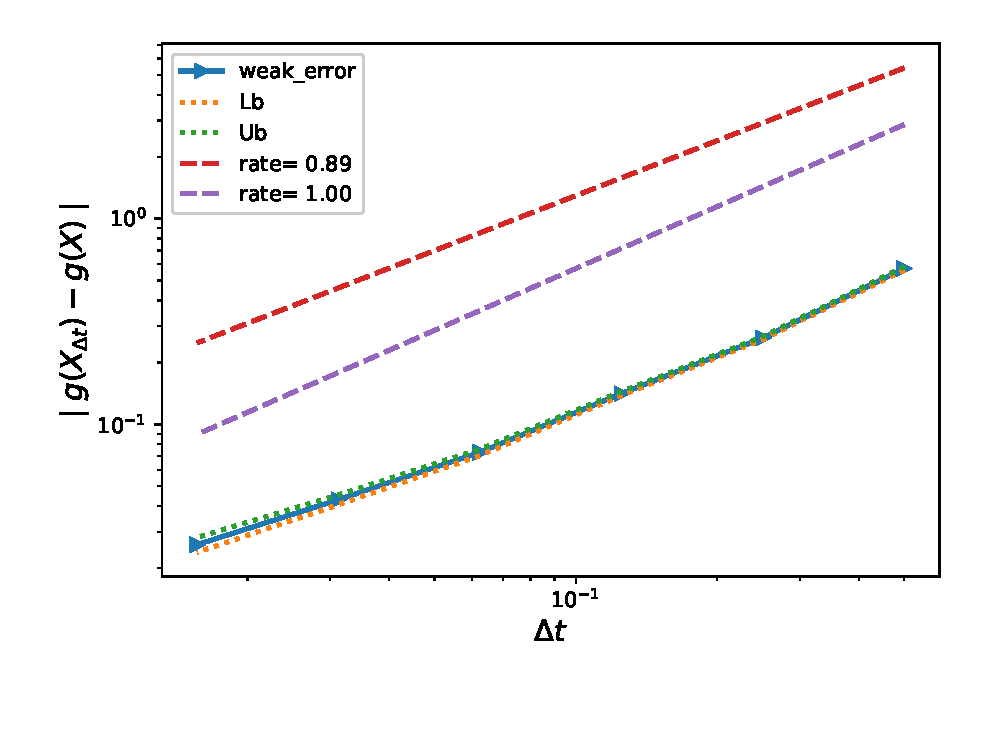
\includegraphics[width=1\linewidth]{./figures/rBergomi_weak_error_rates/without_richardson/H_007/weak_convergence_order_Bergomi_H_007_K_1_M_10_6_CI_relative}
		\caption{}
		\label{fig:sub3}
	\end{subfigure}%
	\begin{subfigure}{.4\textwidth}
		\centering
		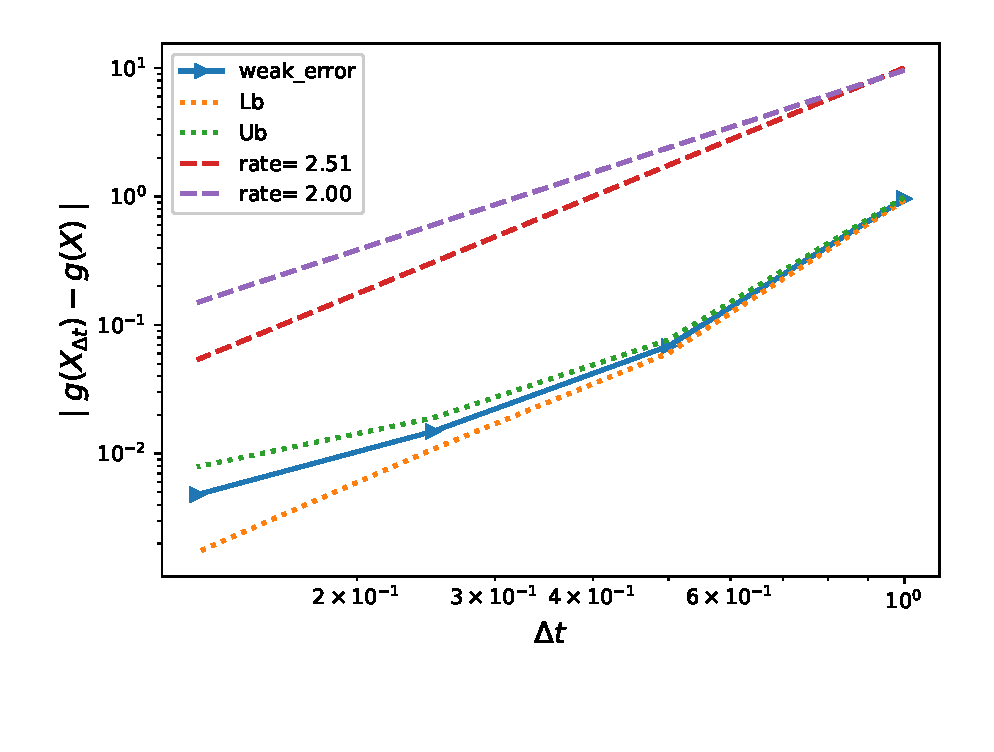
\includegraphics[width=1\linewidth]{./figures/rBergomi_weak_error_rates/with_richardson/H_007/weak_convergence_order_Bergomi_H_007_K_1_richardson_relative_M_10_6}
		\caption{}
		\label{fig:sub4}
	\end{subfigure}
	
	\caption{The  convergence of the weak error $\mathcal{E}_B(N)$, defined in \eqref{eq:total_error}, using MC, for set $1$ parameter in Table \ref{table:Reference solution, using MC with $500$ time steps, of Call option price under rBergomi model, for different parameter constellation.}. We refer to $C_{\text{RB}}$ as $\expt{g(X)}$, and to $C_{\text{RB}}^{N}$ as  $\expt{g(X_{\Delta t})}$. The upper and lower bounds are $95\%$ confidence intervals. a) without Richardson extrapolation.  b) with Richardson extrapolation (level $1$).}
	\label{fig:Weak_rate_set1_set_2_without_rich}
\end{figure}
\FloatBarrier


%
%\begin{figure}[!htb]
%	\centering
%	\begin{subfigure}{.35\textwidth}
%		\centering
%		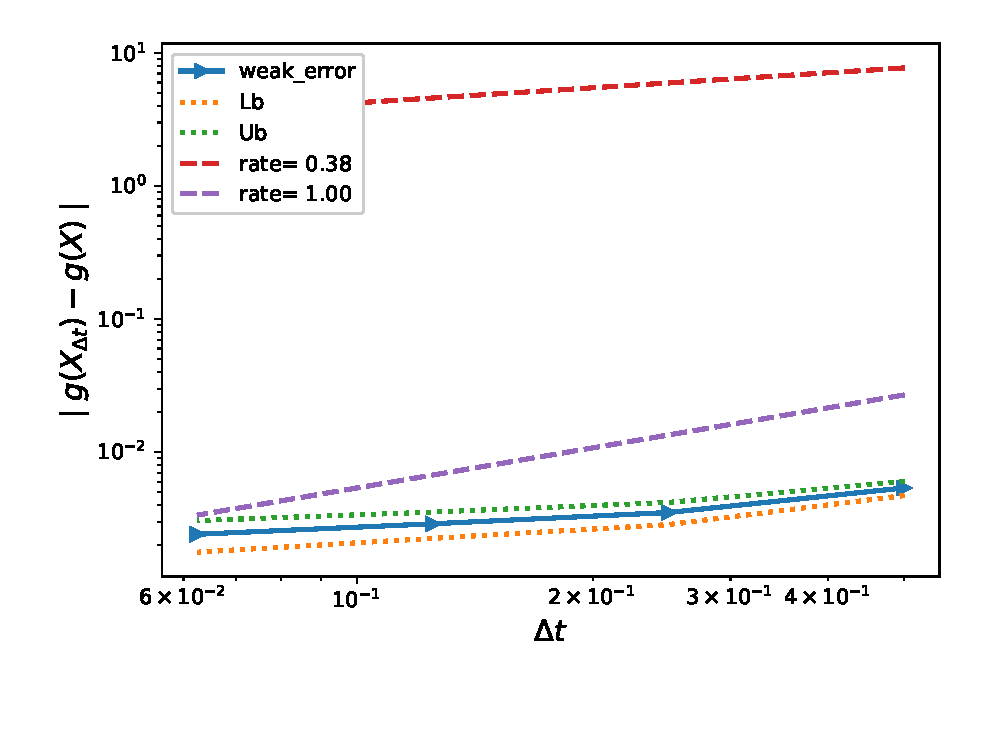
\includegraphics[width=1\linewidth]{./figures/rBergomi_weak_error_rates/without_richardson/H_002/weak_convergence_order_Bergomi_H_002_K_08_M_5_10_6_CI_relative}
%		\caption{}
%		\label{fig:sub3}
%	\end{subfigure}%
%	\begin{subfigure}{.35\textwidth}
%		\centering
%		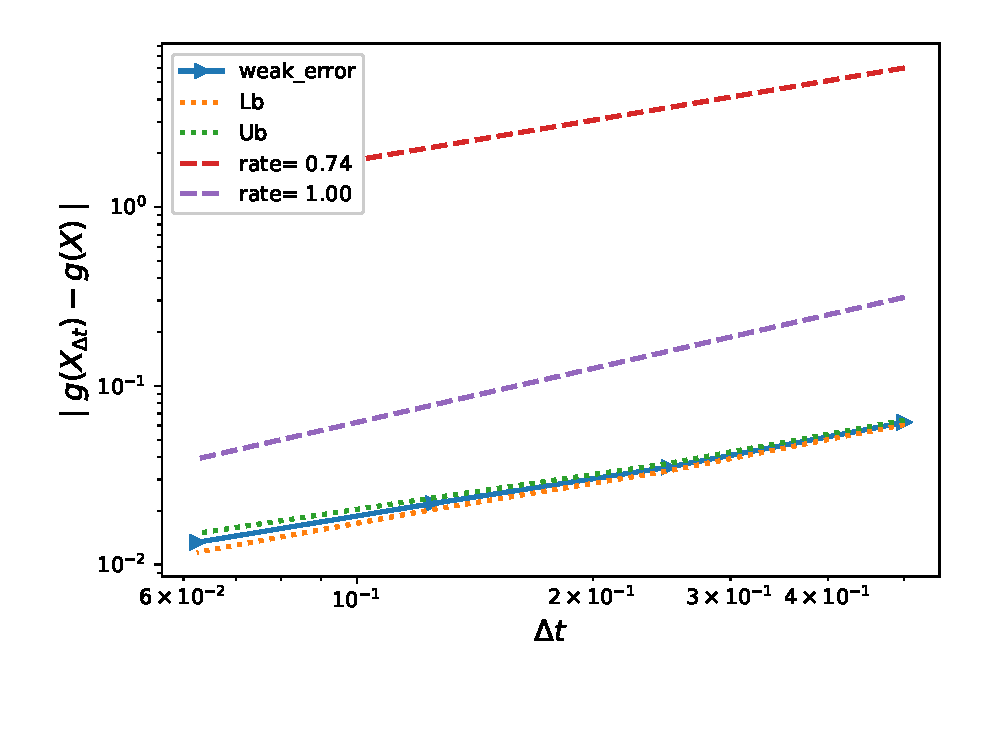
\includegraphics[width=1\linewidth]{./figures/rBergomi_weak_error_rates/without_richardson/H_002/weak_convergence_order_Bergomi_H_002_K_12_M_3_10_6_CI_relative}
%		\caption{}
%		\label{fig:sub4}
%	\end{subfigure}
%	
%	\caption{The rate of convergence of the weak error $\abs{\expt{g(X_{\Delta t})}-g(X)}$  without Richardson extraploation, using MC with $M=5.10^6$: a) Set $3$ parameters in table \ref{table:Reference solution, using MC with $500$ time steps, of Call option price under rBergomi model, for different parameter constellation.},  b) Set $4$ parameters in table \ref{table:Reference solution, using MC with $500$ time steps, of Call option price under rBergomi model, for different parameter constellation.}. }
%	\label{fig:Weak_rate_H_002_without_rich_K_1_K_08}
%\end{figure}

\FloatBarrier









%\begin{figure}[!htb]
%		\centering
%		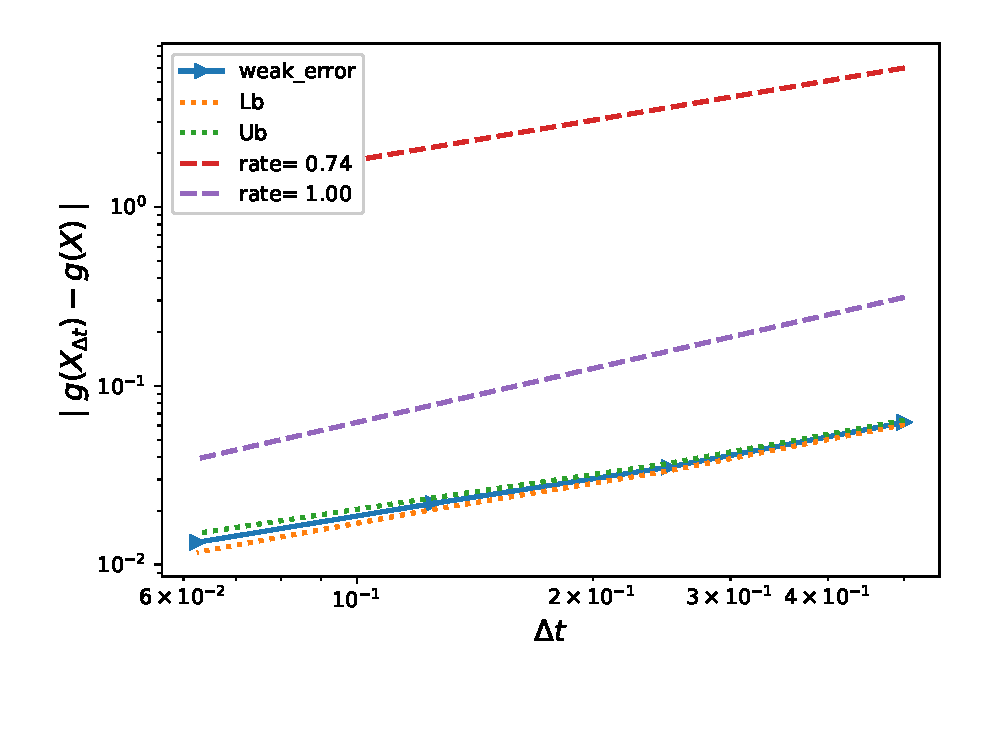
\includegraphics[width=0.35\linewidth]{./figures/rBergomi_weak_error_rates/without_richardson/H_002/weak_convergence_order_Bergomi_H_002_K_12_M_3_10_6_CI_relative}	
%	\caption{The rate of convergence of the weak error $\abs{\expt{g(X_{\Delta t})}-g(X)}$, for set $5$ parameters in table \ref{table:Reference solution, using MC with $500$ time steps, of Call option price under rBergomi model, for different parameter constellation.}, without Richardson extraploation, using MC with $M=5.10^6$.}
%	\label{fig:Weak_rate_H_002_without_rich_K_12}
%\end{figure}




%\subsubsection{With Richardson extrapolation (level 1)}

%\FloatBarrier
%\begin{figure}[h!]
%	\centering
%	\begin{subfigure}{.35\textwidth}
%		\centering
%		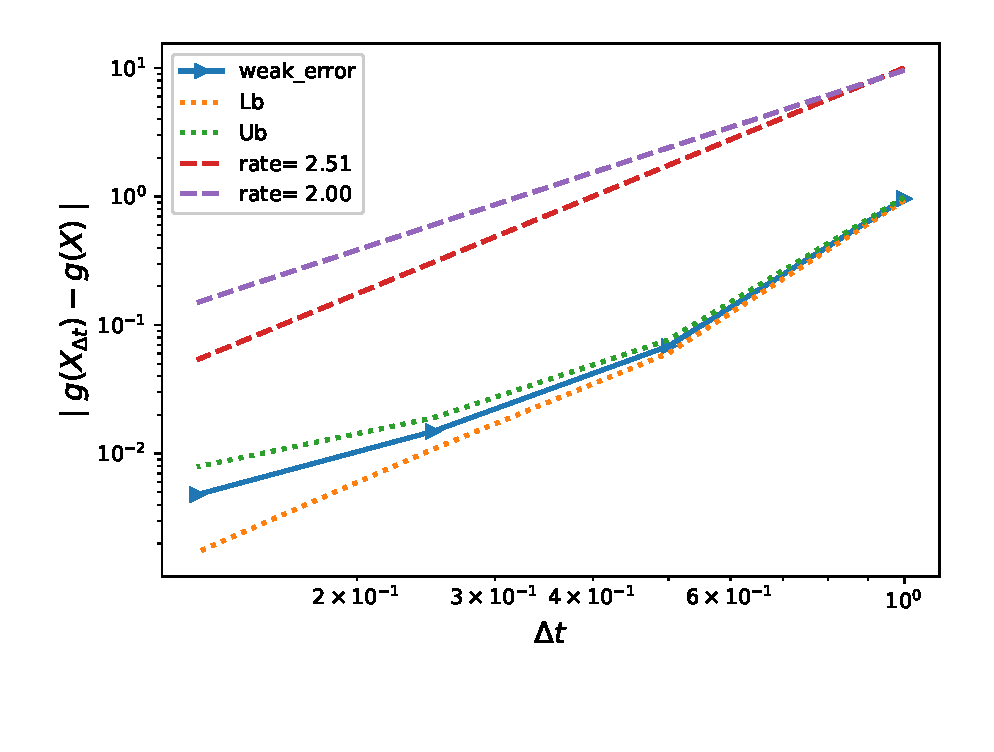
\includegraphics[width=1\linewidth]{./figures/rBergomi_weak_error_rates/with_richardson/H_007/weak_convergence_order_Bergomi_H_007_K_1_richardson_relative_M_10_6}
%		\caption{}
%		\label{fig:sub3}
%	\end{subfigure}%
%	\begin{subfigure}{.35\textwidth}
%		\centering
%		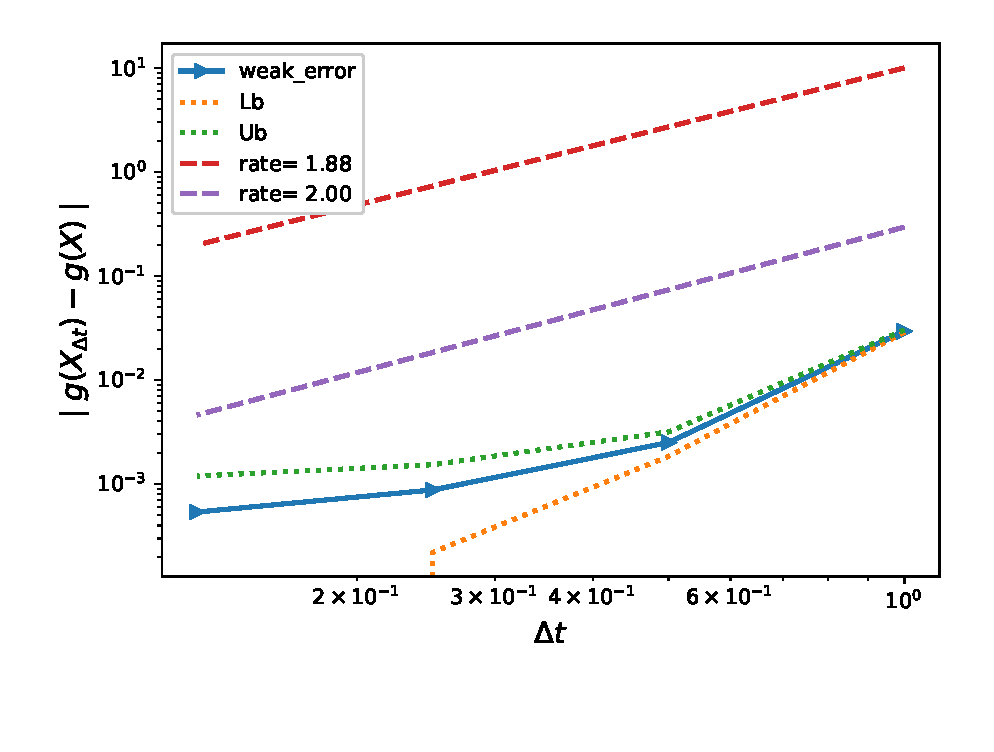
\includegraphics[width=1\linewidth]{./figures/rBergomi_weak_error_rates/with_richardson/H_002/weak_convergence_order_Bergomi_H_002_K_1_M_1_10_7_richardson_relative}
%		\caption{}
%		\label{fig:sub4}
%	\end{subfigure}
%	
%	\caption{The rate of convergence of the weak error  $\abs{\expt{2 g(X_{\Delta t/2}) -g(X_{\Delta t})}-g(X)}$   with Richardson extraploation, using MC with $M=10^6$: a) Set $1$ parameters in table \ref{table:Reference solution, using MC with $500$ time steps, of Call option price under rBergomi model, for different parameter constellation.}.  b) Set $2$ parameters in table \ref{table:Reference solution, using MC with $500$ time steps, of Call option price under rBergomi model, for different parameter constellation.}, }
%	\label{fig:Weak_rate_H_043_007_with_rich}
%\end{figure}
%
%
\FloatBarrier

%\begin{figure}[!htbp]
%	\centering
%		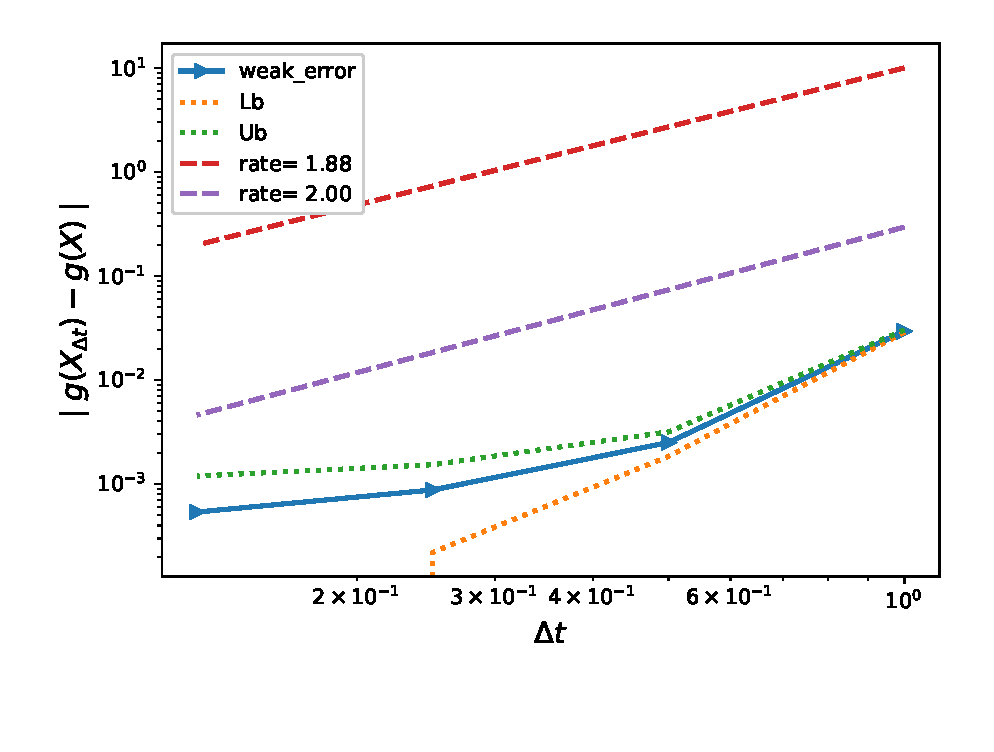
\includegraphics[width=0.35\linewidth]{./figures/rBergomi_weak_error_rates/with_richardson/H_002/weak_convergence_order_Bergomi_H_002_K_1_M_1_10_7_richardson_relative}
%	\caption{The rate of convergence of the weak error $\abs{\expt{2 g(X_{\Delta t/2}) -g(X_{\Delta t})}-g(X)}$,  for set $3$ parameters in table \ref{table:Reference solution, using MC with $500$ time steps, of Call option price under rBergomi model, for different parameter constellation.}, with Richardson extraploation, using MC with $M=10^7$. }
%	\label{fig:Weak_rate_H_002_with_rich_K1}
%\end{figure}
%\FloatBarrier

\subsection{Comparing the different  errors and computational time for MC and MISC}\label{sec:Comparing different  errors and complexity for MC and MISC}
In this section, we conduct a comparison between MC and MISC in terms of errors and computational time. We show tables and plots reporting  the different relative errors involved in the MC method (bias and statistical error\footnote{The statistical error estimate of MC is  $\frac{\sigma_M}{\sqrt{M}}$, which is the standard deviation estimate of the MC estimator,  where $M$ is the number of samples.}  estimates), and in MISC (bias and quadrature error estimates).  While fixing  a  sufficiently small error tolerance in the price estimates,  we also compare the computational time needed for both methods to meet the desired error tolerance.  We note that  in all cases the actual work (runtime) is obtained using an Intel(R) Xeon(R) CPU E$5$-$268$ architecture. 

Through our conducted numerical experiments for each parameter set, we follow these steps to achieve our reported results:

\begin{enumerate}
\item[i)] For a fixed number of time steps, $N$, we compute an accurate estimate, using a large number of samples, $M$, of the biased  MC solution, $C_{RB}^{N}$. This step also provides us with an estimate of the bias error, $\mathcal{E}_B(N)$, defined by \eqref{eq:total_error}. 
\item[ii)] The estimated  biased solution,  $C_{RB}^{N}$, is used as a reference solution  to MISC to compute the quadrature error, $\mathcal{E}_Q(\text{TOL}_{\text{MISC}},N)$, defined by \eqref{eq:quadrature error}.
\item[iii)] In order to compare with MC method, the number of samples, $M$, is chosen so that  the statistical error of the Monte Carlo  method, $\mathcal{E}_S(M)$, satisfies
\begin{align}\label{optimal_number_samples}
\mathcal{E}_S(M)= \mathcal{E}_B(N)=\frac{\mathcal{E}_{\text{tot}}}{2}\COMMA
\end{align}
where $\mathcal{E}_B(N)$ is the bias as defined in \eqref{eq:total_error} and
$\mathcal{E}_{\text{tot}}$ is the total error. 
\end{enumerate}

We show  the summary of our numerical findings in Table \ref{table:Summary of our numerical results.}, which  highlights the computational gains achieved by MISC over MC method to meet a certain error tolerance, which we set approximately to $1\%$. More detailed results for each case of parameter set, as in Table \ref{table:Reference solution, using MC with $500$ time steps, of Call option price under rBergomi model, for different parameter constellation.},  are provided in  Sections \ref{sec:Case of set $2$ parameters_linear}, \ref{sec:Case of set 3 parameters}, \ref{sec:Case of set 4 parameters} and \ref{sec:Case of set 5 parameters}. 
\FloatBarrier
\begin{table}[!h]
	\centering
	\begin{small}
	\begin{tabular}{l*{4}{c}r}
	\toprule[1.5pt]
		Parameter set           & Level of Richardson extrapolation    &  Total relative error  & Ratio of CPU time  $\left(\text{MC}/ \text{MISC} \right)$ \\
		\hline
			Set $1$ & level $1$ &  $3\%$&  $1.6$ \\	
              & level $2$ &  $1\%$ &  $>9$ \\	
              \hline
            Set $2$  & without    &  $0.2\%$&  $5$ \\		
				 \hline
					Set $3$  & without    &  $0.4\%$&  $7$ \\	
					\hline
						Set $4$ & without  &  $2\%$&  $1.3$ \\	
		\bottomrule[1.25pt]
	\end{tabular}
\end{small}
	\caption{Summary of relative errors and computational gains, achieved by the different methods. In this table, we highlight the computational gains achieved by MISC over MC method to meet a certain error tolerance. As expected, these gains are improved when applying Richardson extrapolation as observed for the case of parameters set $1$. We provide details about the way we compute these gains for each case in the following sections.}
	\label{table:Summary of our numerical results.}
\end{table}
\FloatBarrier

	
	



%\subsubsection{Case of set $1$ parameters in table \ref{table:Reference solution, using MC with $500$ time steps, of Call option price under rBergomi model, for different parameter constellation.}}\label{sec:Case of set 1 parameters}
%
%\subsubsection*{Without Richardson extrapolation}
%%\begin{table}[h!]
%%	\centering
%%	\begin{tabular}{l*{6}{c}r}
%%		Method \textbackslash  Steps            & $2$ & $4$ & $8$ & $16$ &   \\
%%		\hline
%%%		MISC ($\text{TOL}_{\text{MISC}}=5.10^{-1}$)  & $0.1140$ & $0.0961$ & $0.0848$ & $0.0781$  \\
%%		MISC ($\text{TOL}_{\text{MISC}}=10^{-1}$)  & $0.1140$ & $0.0961$ & $0.0871$ & $0.0802$  \\
%%%		MISC ($\text{TOL}_{\text{MISC}}=5.10^{-2}$)  & $0.1140$ & $0.0963$ & $0.0843$ & $0.0824$  \\
%%		MISC ($\text{TOL}_{\text{MISC}}=10^{-2}$)  & $0.1077$ & $0.0944$ & $0.0838$ & $0.0772$  \\
%%
%%		MISC ($\text{TOL}_{\text{MISC}}=10^{-3}$)  & $0.1077$ & $0.0921$ & $0.0819$ & $0.0762$  \\
%%%		MISC ($\text{TOL}_{\text{MISC}}=5.10^{-4}$)  & $0.1079   $ & $0.0921$ & $0.0822$ & $0.0762$  \\
%%		MISC ($\text{TOL}_{\text{MISC}}=10^{-4}$)  & $0.1079$ & $0.0921$ & $0.0822$ & $-$  \\
%%		\hline
%%		MC method ($M=8.10^{6}$)   & $  0.1078$ & $ 0.0921
%%		$  & $   0.0822
%%		$ & $ 0.0767$ \\		
%%		
%%		\hline
%%	\end{tabular}
%%	\caption{ Call option price of the different methods for different number of time steps. Case of set $1$ parameters in table \ref{table:Reference solution, using MC with $500$ time steps, of Call option price under rBergomi model, for different parameter constellation.}, without Richardson extrapolation.}
%%	\label{table: Call option price of the different methods for different number of time steps. Case set 1}
%%\end{table}
%
%
%\begin{table}[h!]
%	\centering
%	\begin{tabular}{l*{6}{c}r}
%		Method \textbackslash  Steps            & $2$ & $4$ & $8$ & $16$  \\
%		\hline
%		MC Bias ($M=8.10^6$)   & 	$ \underset{( 0.0366)}{\mathbf{0.5142}}$  & $\underset{( 0.0209)}{\mathbf{0.2933}}$  & $\underset{( 0.0110)}{\mathbf{0.1551}}$ & $\underset{( 0.0055)}{\mathbf{0.0777}}$\\ 
%		
%		MC Statistical error ($M=8.10^6$)  &  $\underset{(  6.0e-05)} {\mathbf{8.4e-04}}$  & $\underset{(3.4e-05)} {\mathbf{4.8e-04}}$  & $\underset{(2.7e-05)} {\mathbf{ 3.8e-04}}$ & $\underset{( 2.35e-05)} {\mathbf{3.3e-04}}$	\\
%
%		\hline
%	\end{tabular}
%	\caption{Bias and statistical errors of MC  for computing call option price  for different number of time steps. Case set $1$, without Richardson extrapolation. The numbers between parentheses are the corresponding absolute errors.}
%	\label{Bias and Statistical errors of MC ($M=10^6$)  for computing Call option price  for different number of time steps. Case set 1, without Richardson extrapolation. The numbers between parentheses are the corresponding absolute errors.}
%\end{table}
%
%
%
%
%
%
%\FloatBarrier
%
%\begin{figure}[h!]
%	\centering
%	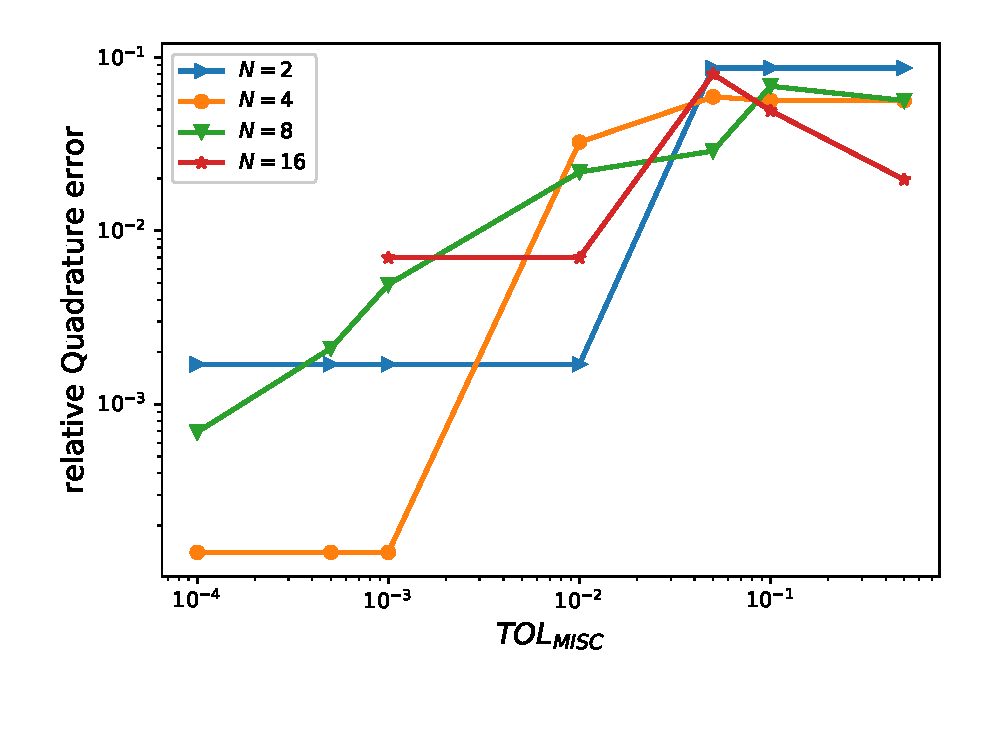
\includegraphics[width=0.35\linewidth]{./figures/rBergomi_MISC_quadratre_error/vs_TOL/set1/relative_quad_error_wrt_MISC_TOL_set1_non_rich}
%	
%	
%	\caption{Quadrature error of MISC, with different tolerances, to compute call option price for different number of time steps. Case  set $1$ parameters, without Richardson extrapolation. See detailed values  in table \ref{Quadrature error of MISC to compute Call option price of the different tolerances for different number of time steps. Case  set $1$ parameters, without Richardson extrapolation. The numbers between parentheses are the corresponding absolute errors.}}
%	\label{fig:Quadrature_error_set1}
%\end{figure}
%
%\FloatBarrier
%
%
%\begin{table}[h!]
%	\centering
%	\begin{tabular}{l*{6}{c}r}
%		Method \textbackslash  Steps            & $2$ & $4$ & $8$ & $16$  \\
%		\hline
%%		MISC ($\text{TOL}_{\text{MISC}}=5.10^{-1}$)  & $\mathbf{0.6010}$ & $\mathbf{0.3496}$ & $\mathbf{ 0.2114}$ & $\mathbf{ 0.0974}$  \\
%		MISC ($\text{TOL}_{\text{MISC}}=10^{-1}$)  & $\mathbf{0.6010}$ & $\mathbf{0.3496}$ & $\mathbf{  0.2232}$ & $\mathbf{
%			0.1269}$  \\
%%		MISC ($\text{TOL}_{\text{MISC}}=5.10^{-2}$)  &$\mathbf{0.6010}$ & $\mathbf{  0.3524}$ & $\mathbf{ 0.1839}$ & $\mathbf{  0.1577}$  \\
%		MISC ($\text{TOL}_{\text{MISC}}=10^{-2}$)  & $\mathbf{\red{0.5159}}$ & $\mathbf{0.3257}$ & $\mathbf{ 0.1769}$ & $\mathbf{  \red{0.0847}}$  \\
%		MISC ($\text{TOL}_{\text{MISC}}=10^{-3}$)  & $\mathbf{0.5159}$ & $\mathbf{\red{0.2934}}$ & $\mathbf{0.1600}$ & $\mathbf{0.0847}$  \\
%%		MISC ($\text{TOL}_{\text{MISC}}=5.10^{-4}$)  & $\mathbf{0.5159}$ & $\mathbf{0.2934}$ & $\mathbf{0.1572}$ & $\mathbf{-}$  \\
%		MISC ($\text{TOL}_{\text{MISC}}=10^{-4}$)  & $\mathbf{0.5159}$ & $\mathbf{0.2934}$ & $\mathbf{\red{0.1558}}$ & $\mathbf{-}$  \\
%		\hline
%		MC     & $\mathbf{\red{0.5159}}$ & $\mathbf{\red{0.2938}}$ & $\mathbf{\red{0.1555}}$ &$\mathbf{  \red{0.0817}}$  \\	
%		
%		\hline
%	\end{tabular}
%	\caption{Total relative error of MISC, with different tolerances,  and MC to compute call option price for different number of time steps. Case  set $1$ parametrs of table \ref{table:Reference solution, using MC with $500$ time steps, of Call option price under rBergomi model, for different parameter constellation.}, without Richardson extrapolation. The values marked in red, for MISC method, correspond to the total relative errors associated with  stable quadrature errors for MISC, and will be used for complexity comparison against MC.}
%	\label{Total error of MISC and MC to compute Call option price of the different tolerances for different number of time steps. Case set 1, without Richardson extrapolation. The numbers between parentheses are the corresponding absolute errors.}
%\end{table}
%
%
%
%\begin{table}[h!]
%	\centering
%	\begin{tabular}{l*{6}{c}r}
%		Method \textbackslash  Steps            & $2$ & $4$ & $8$ & $16$ &   \\
%		\hline
%%		MISC ($\text{TOL}_{\text{MISC}}=5.10^{-1}$)  & $0.1$ & $0.1$ & $0.2$ & $0.4$  \\
%		MISC ($\text{TOL}_{\text{MISC}}=10^{-1}$)  & $0.1$ & $0.1$ & $0.6$ & $6$  \\
%%		MISC ($\text{TOL}_{\text{MISC}}=5.10^{-2}$)  & $0.1$ & $0.3$ & $2$ & $14$  \\
%		MISC ($\text{TOL}_{\text{MISC}}=10^{-2}$)  & $\red{0.2}$ & $1$ & $9$ & $\red{215}$  \\
%		MISC ($\text{TOL}_{\text{MISC}}=10^{-3}$)  & $2$ & $\red{11}$ & $243$ & $4650$  \\
%%		MISC ($\text{TOL}_{\text{MISC}}=5.10^{-4}$)  & $3$ & $17$ & $ 670$ & $-$  \\
%		MISC ($\text{TOL}_{\text{MISC}}=10^{-4}$)  & $6$ & $96$ & $\red{5760}$ & $-$  \\
%		\hline
%		MC     & $\red{ 50}$  & $\red{344}$  & $\red{637}$ & $\red{8}$  \\
%		
%		\hline
%		Ratio of $\left(\text{MC}/ \text{MISC} \right)$  &$\red{  250}$ & $\red{    31
%		}$  & $\red{ 0.1
%		}$  & $\red{  0.04}$ \\
%		\hline
%	\end{tabular}
%	\caption{Comparison of the computational time (in Seconds) of  MC and MISC, used to compute call option price of the rBergomi model for different number of time steps. Case set $1$ parametrs of table \ref{table:Reference solution, using MC with $500$ time steps, of Call option price under rBergomi model, for different parameter constellation.}. The
%		average MC CPU time is computed over 10 runs. }
%	\label{Comparison of the computational time of  MC and MISC, used to compute Call option price of rBergomi model for different number of time steps. Case set1}
%\end{table}
%
%\FloatBarrier
%\subsubsection*{With Richardson extrapolation (level $1$)}
%
%
%
%
%
%
%
%%\begin{table}[h!]
%%	\centering
%%	\begin{tabular}{l*{6}{c}r}
%%		Method \textbackslash  Steps    &$1-2$         & $2-4$ & $4-8$ \\
%%		\hline
%%%		MISC ($\text{TOL}_{\text{MISC}}=5.10^{-1}$)& $0.1357$  & $0.0783$ & $0.0735$ \\
%%		MISC ($\text{TOL}_{\text{MISC}}=10^{-1}$)  &$0.1357$  &$0.0783$ & $0.0785$   \\
%%%		MISC ($\text{TOL}_{\text{MISC}}=5.10^{-2}$)  & $0.1357$ & $0.0831$ & $0.0773$   \\
%%		MISC ($\text{TOL}_{\text{MISC}}=10^{-2}$)  & $0.1237$ &$0.0781$ & $0.0745$   \\
%%
%%		MISC ($\text{TOL}_{\text{MISC}}=10^{-3}$)  & $0.1224$ &$0.0766$ & $0.0720$  \\
%%%		MISC ($\text{TOL}_{\text{MISC}}=10^{-4}$)  &$0.1224$ & $0.0763$ & $0.0724$ \\
%%		\hline
%%		MC method ($M=10^6$)  &$	0.1237$ & $0.0752$ & $0.0721$ \\
%%		\hline
%%	\end{tabular}
%%	\caption{Call option price of the different methods for different number of time steps. Case set $1$ parameters of table \ref{table:Reference solution, using MC with $500$ time steps, of Call option price under rBergomi model, for different parameter constellation.}, using Richardson extrapolation (level $1$).}
%%	\label{table:  Call option price of the different methods for different number of time steps. Case set $1$ parameter, using Richardson extrapolation (level $1$)}
%%\end{table}
%
%
%
%
%\begin{table}[h!]
%	\centering
%	\begin{tabular}{l*{6}{c}r}
%		Method \textbackslash  Steps            & $1-2$ & $2-4$ & $4-8$ & $8-16$  \\
%		\hline
%		MC  Bias ($M=10^6$)    &$\underset{( 0.0525)}{\mathbf{0.7378}}$  & $\underset{(    0.0040)}{\mathbf{0.0561}}$  & $\underset{(0.0009 )}{\mathbf{0.0127}}$  & $\underset{(0.0001)}{\mathbf{0.0021}}$ \\	
%		
%		MC Statistical error ($M=10^6$)   & $\underset{( 2.3e-04)}{\mathbf{3.3e-03}}$  & $\underset{(  1.1e-04)}{\mathbf{1.6e-03}}$  & $\underset{(7.1e-05)}{\mathbf{1.0e-03}}$ & $\underset{(   6.4e-05 )}{\mathbf{9.0e-04}}$ \\	
%		
%		
%		\hline
%	\end{tabular}
%	\caption{Bias and statistical errors of MC   for computing call option price  for different number of time steps. Case set $1$ parameters in tabel \ref{table:Reference solution, using MC with $500$ time steps, of Call option price under rBergomi model, for different parameter constellation.}, with Richardson extrapolation (level $1$). The numbers between parentheses are the corresponding absolute errors.}
%	\label{Bias and Statistical errors of MC ($M=10^6$)  for computing Call option price  for different number of time steps. Case set $1$ parameters, with Richardson extrapolation (level1). The numbers between parentheses are the corresponding absolute errors.}
%\end{table}
%
%
%
%
%
%
%
%
%\begin{figure}[h!]
%	\centering
%	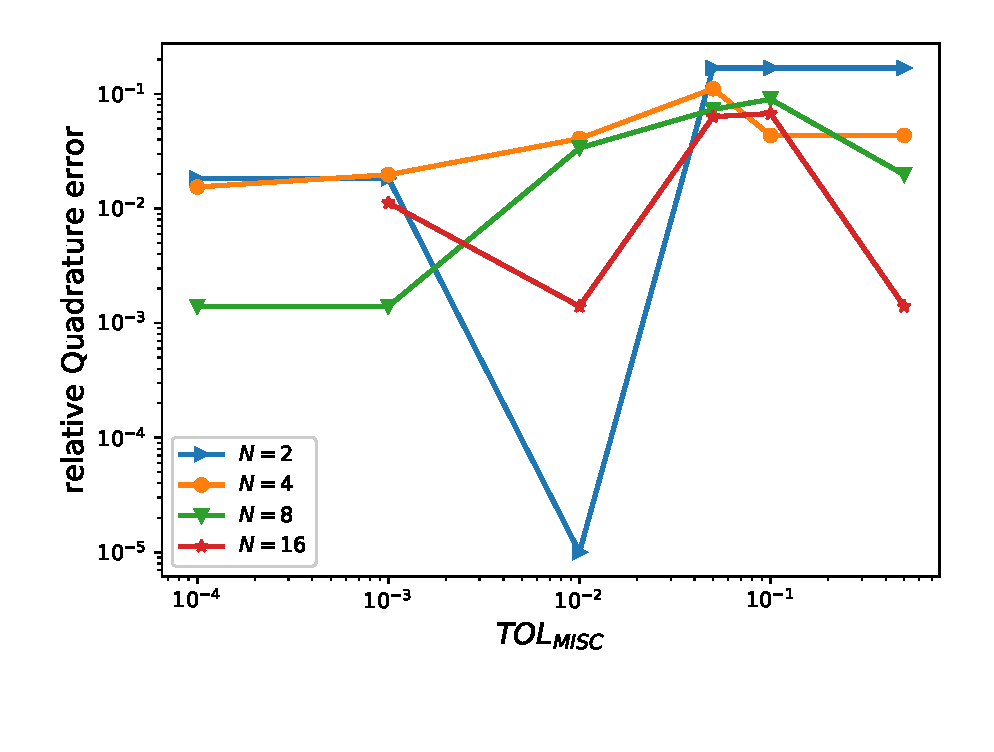
\includegraphics[width=0.35\linewidth]{./figures/rBergomi_MISC_quadratre_error/vs_TOL/set1/relative_quad_error_wrt_MISC_TOL_set1_with_rich}
%	
%	
%	\caption{Quadrature error of MISC, with different tolerances, to compute call option price for different number of time steps. Case  set $1$ parameters, with Richardson extrapolation.  See detailed values  in table \ref{Quadrature error of MISC to compute Call option price of the different tolerances for different number of time steps. Case set $1$ parameters, with Richardson extrapolation(level $1$). The numbers between parentheses are the corresponding absolute errors.}.}
%\end{figure}
%
%
%
%\begin{table}[!h]
%	\centering
%	\begin{tabular}{l*{6}{c}r}
%		Method \textbackslash  Steps            & $1-2$ & $2-4$ & $4-8$   \\
%		\hline
%%		MISC ($\text{TOL}_{\text{MISC}}=5.10^{-1}$)  & $\mathbf{0.9063
%%		}$ & $\mathbf{ 0.0996}$ & $\mathbf{0.0324
%%		}$  \\
%		MISC ($\text{TOL}_{\text{MISC}}=10^{-1}$)  & $\mathbf{0.9063
%		}$ & $\mathbf{ 0.0996}$ & $\mathbf{  0.1026}$   \\
%%		MISC ($\text{TOL}_{\text{MISC}}=5.10^{-2}$)  & $\mathbf{0.9063
%%		}$ & $\mathbf{    0.1670}$ & $\mathbf{ 0.0857}$  \\
%		MISC ($\text{TOL}_{\text{MISC}}=10^{-2}$)  & $\mathbf{0.7378}$ & $\mathbf{  0.0968}$ & $\mathbf{   0.0464}$  \\	
%		MISC ($\text{TOL}_{\text{MISC}}=10^{-3}$)  & $\mathbf{\red{0.7561}}$ & $\mathbf{\red{0.0758}}$ & $\mathbf{\red{0.0141}}$  \\
%%		MISC ($\text{TOL}_{\text{MISC}}=10^{-4}$)  & $\mathbf{0.7561}$ & $\mathbf{0.0715}$ & $\mathbf{0.0141}$ \\
%		\hline
%		MC   & $\mathbf{\red{0.7561}}$  & $\mathbf{\red{0.0758}}$  & $\mathbf{\red{0.0141}}$  \\
%		
%		\hline
%	\end{tabular}
%	\caption{Total  relative error of MISC and MC, with different tolerances, to compute call option price for different number of time steps. Case set $1$ parameters in table \ref{table:Reference solution, using MC with $500$ time steps, of Call option price under rBergomi model, for different parameter constellation.}, with Richardson extrapolation(level $1$). The values marked in red, for MISC method, correspond to the total relative errors associated with  stable quadrature errors for MISC, and will be used for complexity comparison against MC.}
%	\label{Total  error of MISC and MC to compute Call option price of the different tolerances for different number of time steps. Case set $1$ parameters, with Richardson extrapolation(level $1$). The numbers between parentheses are the corresponding absolute errors.}
%\end{table}
%\FloatBarrier
%\begin{table}[!h]
%	\centering
%	\begin{tabular}{l*{6}{c}r}
%		Method \textbackslash  Steps            & $1-2$ & $2-4$ & $4-8$   \\
%		\hline
%%		MISC ($\text{TOL}_{\text{MISC}}=5.10^{-1}$)  & $0.1$ & $0.1$ & $0.2$  \\
%		MISC ($\text{TOL}_{\text{MISC}}=10^{-1}$)  & $0.1$ & $0.1$ & $0.6$ \\
%%		MISC ($\text{TOL}_{\text{MISC}}=5.10^{-2}$)  & $0.1$ & $0.4$ & $2$   \\
%		MISC ($\text{TOL}_{\text{MISC}}=10^{-2}$)  & $1$ & $2$ & $18$   \\
%		MISC ($\text{TOL}_{\text{MISC}}=10^{-3}$)  & $\red{4}$ & $\red{12}$ & $\red{520}$   \\	
%%		MISC ($\text{TOL}_{\text{MISC}}=10^{-4}$)  & $7$ & $191$ & $7650$  \\
%		\hline
%		MC   & $\red{ 34.7}$  & $\red{37}$  & $ \red{532}$    \\
%		
%		\hline
%		Ratio of $\left(\text{MC}/ \text{MISC} \right)$  &$\red{8.7}$ & $\red{   3.1
%		}$  & $\red{1}$ \\
%		\hline
%	\end{tabular}
%	\caption{Comparison of the computational time (in Seconds) of  MC and MISC, using Richardson extrapolation (level $1$), used to compute call option price of the rBergomi model for different number of time steps. Case set $1$ parameters in table \ref{table:Reference solution, using MC with $500$ time steps, of Call option price under rBergomi model, for different parameter constellation.}. The
%		average MC CPU time is computed over 10 runs.}
%	\label{Comparsion of the computational time of  MC and MISC, using Richardson extrapolation (level $1$), used to compute Call option price of rBergomi model for different number of time steps. Case set $1$ parameters}
%\end{table}
%
%
%
%
%\FloatBarrier
%
%\subsubsection*{With Richardson extrapolation (level $2$)}
%%\FloatBarrier
%%\begin{table}[h!]
%%	\centering
%%	\begin{tabular}{l*{6}{c}r}
%%		Method \textbackslash  Steps           &$1-2-4$ & $2-4-8$ \\
%%		\hline
%%%		MISC ($\text{TOL}_{\text{MISC}}=5.10^{-1}$)& $0.0591$  & $0.0719$ \\
%%		
%%		MISC ($\text{TOL}_{\text{MISC}}=10^{-1}$)  &$0.0567$  &$0.0747$   \\
%%%		MISC ($\text{TOL}_{\text{MISC}}=5.10^{-2}$)  & $0.0733$ & $0.0782$  \\
%%		MISC ($\text{TOL}_{\text{MISC}}=10^{-2}$)  & $		0.0639$ & $0.0729$   \\
%%		MISC ($\text{TOL}_{\text{MISC}}=5.10^{-3}$)  & $	0.0620$ & $0.0708$   \\
%%%		MISC ($\text{TOL}_{\text{MISC}}=10^{-3}$)  & $	0.0608$ & $0.0708$  \\
%%%		MISC ($\text{TOL}_{\text{MISC}}=10^{-4}$)  & $	0.0608$ & $-$   \\
%%		\hline
%%		MC ($M=3.10^6$)  & $0.0608$ & $0.0710$   \\
%%		\hline 
%%	\end{tabular}
%%	\caption{ Call option price of the different methods for different number of time steps.  Case set $1$ parameters in table \ref{table:Reference solution, using MC with $500$ time steps, of Call option price under rBergomi model, for different parameter constellation.}, using Richardson extrapolation (level $2$).}
%%	\label{table: Call option price of the different methods for different number of time steps. Case $K=1$, using Richardson extrapolation_level2}
%%\end{table}
%
%\FloatBarrier
%
%
%\begin{table}[h!]
%	\centering
%	\begin{tabular}{l*{6}{c}r}
%		Method \textbackslash  Steps            & $1-2-4$ & $2-4-8$  \\
%		\hline
%		MC  Bias ($M=3.10^6$)     &$\underset{( 0.0104)}{\mathbf{ 0.1459}}$  & $\underset{(    1.7e-04)}{\mathbf{0.0024}}$   \\	
%		
%		MC Statistical error ($M=3.10^6$)   & $\underset{( 1.0e-04)}{\mathbf{1.5e-03}}$  & $\underset{(   4.8e-05)}{\mathbf{    6.8e-04}}$  \\	
%		
%		
%		
%		\hline
%	\end{tabular}
%	\caption{Bias and statistical errors of MC   for computing call option price  for different number of time steps. Case set $1$ parameters in tabel \ref{table:Reference solution, using MC with $500$ time steps, of Call option price under rBergomi model, for different parameter constellation.}, with Richardson extrapolation (level $2$). The numbers between parentheses are the corresponding absolute errors.}
%	\label{Bias and Statistical errors of MC ($M=3.10^6$)  for computing Call option price  for different number of time steps. Case set $1$ parameters, with Richardson extrapolation (level2). The numbers between parentheses are the corresponding absolute errors.}
%\end{table}
%
%
%
%
%\FloatBarrier
%\begin{figure}[h!]
%	\centering
%	evel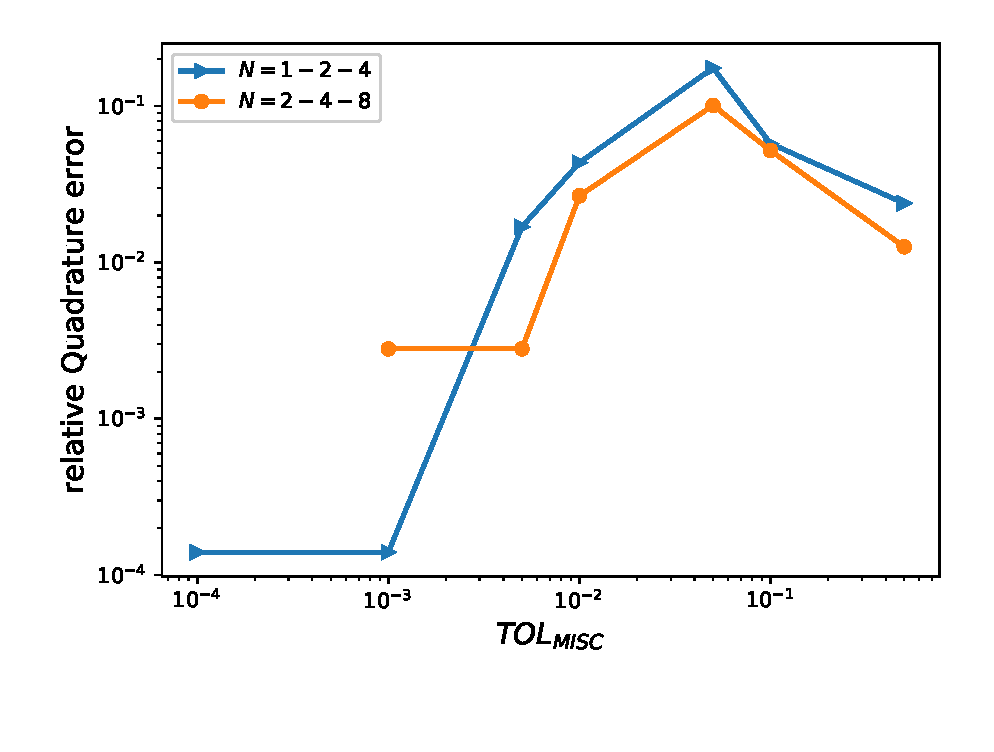
\includegraphics[width=0.35\linewidth]{./figures/rBergomi_MISC_quadratre_error/vs_TOL/set1/relative_quad_error_wrt_MISC_TOL_set1_rich_level2}
%	
%	
%	\caption{Quadrature error of MISC, with different tolerances, to compute call option price of the different tolerances for different number of time steps. Case  set $1$ parameters, with Richardson extrapolation (level $2$).  See detailed values  in table \ref{Quadrature error of MISC to compute Call option price of the different tolerances for different number of time steps. Case set $1$ parameters, with Richardson extrapolation(level $2$). The numbers between parentheses are the corresponding absolute errors.}.}
%	\label{fig:Quadrature_error_set1_rich_level2}
%\end{figure}
%
%
%
%\FloatBarrier
%\begin{table}[!h]
%	\centering
%	\begin{tabular}{l*{6}{c}r}
%		Method \textbackslash  Steps            & $1-2-4$ & $2-4-8$  \\
%		\hline
%%		MISC ($\text{TOL}_{\text{MISC}}=5.10^{-1}$)  & $\mathbf{0.1698
%%		}$ & $\mathbf{ 0.0150}$  \\
%		MISC ($\text{TOL}_{\text{MISC}}=10^{-1}$)  & $\mathbf{0.2035
%		}$ & $\mathbf{ 0.0544}$ \\
%%		MISC ($\text{TOL}_{\text{MISC}}=5.10^{-2}$)  & $\mathbf{0.3214
%%		}$ & $\mathbf{    0.1035}$  \\
%		MISC ($\text{TOL}_{\text{MISC}}=10^{-2}$)  & $\mathbf{0.1894}$ & $\mathbf{  0.0291}$   \\	
%		MISC ($\text{TOL}_{\text{MISC}}=5.10^{-3}$)  & $\mathbf{\red{0.1628}}$ & $\mathbf{\red{0.0052}}$   \\
%%		MISC ($\text{TOL}_{\text{MISC}}=10^{-3}$)  & $\mathbf{0.1460}$ & $\mathbf{0.0052}$   \\
%%		MISC ($\text{TOL}_{\text{MISC}}=10^{-4}$)  & $\mathbf{0.1460}$ & $\mathbf{-}$  \\
%		\hline
%		MC   & $\mathbf{\red{0.1628}}$  & $\mathbf{\red{0.0052}}$    \\
%		\hline
%	\end{tabular}
%	\caption{Total  relative error of MISC, with different tolerances, and MC to compute call option price for different number of time steps. Case set $1$ parameters in table \ref{table:Reference solution, using MC with $500$ time steps, of Call option price under rBergomi model, for different parameter constellation.}, with Richardson extrapolation(level $2$). The values marked in red, for MISC method, correspond to the total relative errors associated with  stable quadrature errors for MISC, and will be used for complexity comparison against MC.}
%	\label{Total  error of MISC and MC to compute Call option price of the different tolerances for different number of time steps. Case set $1$ parameters, with Richardson extrapolation(level $2$). The numbers between parentheses are the corresponding absolute errors.}
%\end{table}
%
%\FloatBarrier
%
%\begin{table}[!h]
%	\centering
%	\begin{tabular}{l*{6}{c}r}
%		Method \textbackslash  Steps            & $1-2-4$ & $2-4-8$   \\
%		\hline
%%		MISC ($\text{TOL}_{\text{MISC}}=5.10^{-1}$)  & $0.2$ & $0.3$  \\
%		MISC ($\text{TOL}_{\text{MISC}}=10^{-1}$)  & $0.25$ & $2$ &   \\
%%		MISC ($\text{TOL}_{\text{MISC}}=5.10^{-2}$)  & $0.55$ & $5$  \\
%		MISC ($\text{TOL}_{\text{MISC}}=10^{-2}$)  & $2$ & $24$   \\
%		MISC ($\text{TOL}_{\text{MISC}}=5.10^{-3}$)  & $\red{5}$ & $\red{64}$  \\	
%%		MISC ($\text{TOL}_{\text{MISC}}=10^{-3}$)  & $24$ & $1067$  \\	
%%		MISC ($\text{TOL}_{\text{MISC}}=10^{-4}$)  & $ 233$ & $-$   \\
%		\hline
%		MC    & $\red{20}$  & $\red{231}$  \\
%		
%		\hline
%		Ratio of $\left(\text{MC}/ \text{MISC} \right)$  &$\red{4}$ & $\red{  3.6}$   \\
%		\hline
%	\end{tabular}
%	\caption{Comparison of the computational time (in Seconds) of  MC and MISC, using Richardson extrapolation (level $2$), used to compute call option price of the rBergomi model for different number of time steps. Case set $1$ parameters in table \ref{table:Reference solution, using MC with $500$ time steps, of Call option price under rBergomi model, for different parameter constellation.}. The
%		average MC CPU time is computed over 10 runs.}
%	\label{Comparsion of the computational time of  MC and MISC, using Richardson extrapolation (level $2$), used to compute Call option price of rBergomi model for different number of time steps. Case set $1$ parameters}
%\end{table}
%
%
%
%\FloatBarrier
%
%
%
%
%
%
%
%\begin{figure}[h!]
%	\centering
%	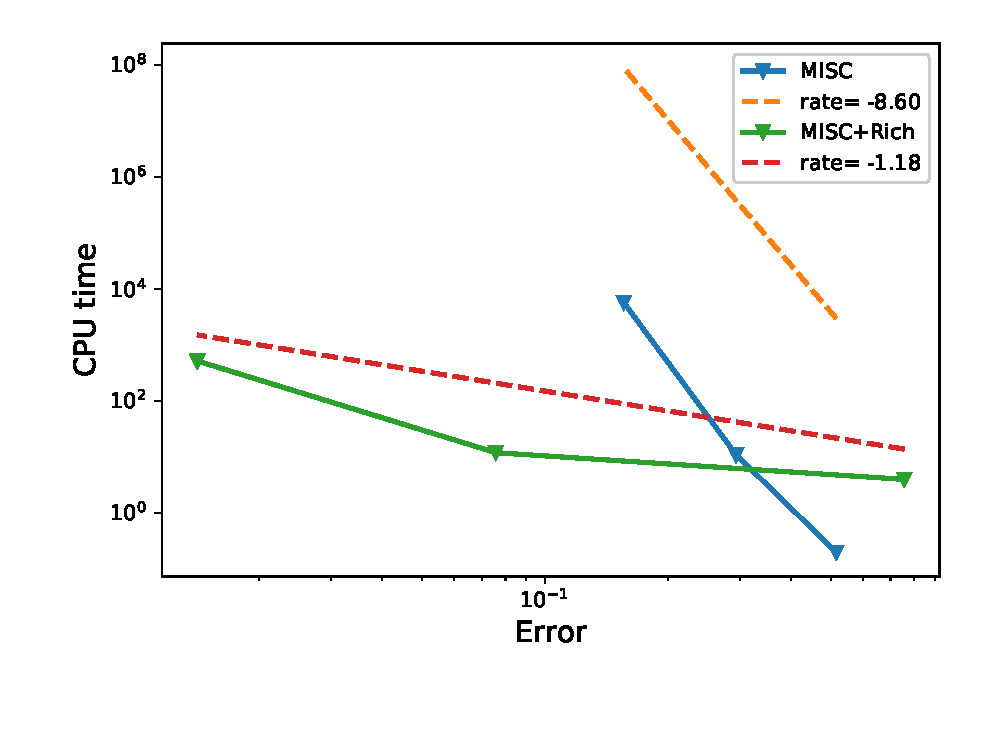
\includegraphics[width=0.35\linewidth]{./figures/rBergomi_Complexity_rates/set1/error_vs_time_set1_comparison}
%	
%	\caption{Complexity plot for  MISC (with and without) Richardson extrapolation for case set $1$ parameters of table \ref{table:Reference solution, using MC with $500$ time steps, of Call option price under rBergomi model, for different parameter constellation.}.}
%	\label{fig:Complexity plot for  MISC for Case set $1$ parameters, comparison}
%\end{figure}
%
%\FloatBarrier
%
%
%


\subsubsection{Case of parameters in Set 1, in Table \ref{table:Reference solution, using MC with $500$ time steps, of Call option price under rBergomi model, for different parameter constellation.} }
\label{sec:Case of set $2$ parameters_linear}

In this section, we conduct our numerical experiments for three different scenarios: i) without Richardson extrapolation (see Tables \ref{Total error of MISC and MC to compute Call option price of the different tolerances for different number of time steps. Case $K=1$, $H=0.07$, without Richardson extrapolation. The numbers between parentheses are the corresponding absolute errors,linear} and \ref{Comparsion of the computational time of  MC and MISC, used to compute Call option price of rBergomi model for different number of time steps. Case $K=1, H=0.07$, linear}), ii) with (level $1$) Richardson extrapolation (see Tables \ref{Total  error of MISC and MC to compute Call option price of the different tolerances for different number of time steps. Case set $2$ parameters, with Richardson extrapolation(level $1$). The numbers between parentheses are the corresponding absolute errors,relative} and \ref{Comparsion of the computational time of  MC and MISC, using Richardson extrapolation (level $1$), used to compute Call option price of rBergomi model for different number of time steps. Case set $2$ parameters,linear}), and iii) with (level $2$) Richardson extrapolation (see Tables \ref{Total  error of MISC and MC to compute Call option price of the different tolerances for different number of time steps. Case set $2$ parameters, with Richardson extrapolation(level $2$). The numbers between parentheses are the corresponding absolute errors,linear} and \ref{Comparsion of the computational time of  MC and MISC, using Richardson extrapolation (level $2$), used to compute Call option price of rBergomi model for different number of time steps. Case set $2$ parameters,linear}).  Our numerical experiments show that  MISC coupled with (level $1$) Richardson extrapolation  requires  approximately $60\%$ of the work of MC coupled with (level $1$) Richardson extrapolation, to achieve  a total relative error of around $3\%$. This gain is improved further  when applying level $2$ Richardson extrapolation. In fact,  MISC coupled with (level $2$)  Richardson extrapolation requires  approximately less than $10\%$ of the work of MC coupled with (level $2$)  Richardson extrapolation, to achieve  a total relative error below  $1\%$. Applying Richardson extrapolation brought a significant improvement for MISC (see Figure \ref{fig:Complexity plot for  MISC for Case set $2$ parameters, comparison} and  Tables \ref{Total error of MISC and MC to compute Call option price of the different tolerances for different number of time steps. Case $K=1$, $H=0.07$, without Richardson extrapolation. The numbers between parentheses are the corresponding absolute errors,linear},\ref{Comparsion of the computational time of  MC and MISC, used to compute Call option price of rBergomi model for different number of time steps. Case $K=1, H=0.07$, linear},\ref{Total  error of MISC and MC to compute Call option price of the different tolerances for different number of time steps. Case set $2$ parameters, with Richardson extrapolation(level $1$). The numbers between parentheses are the corresponding absolute errors,relative},\ref{Comparsion of the computational time of  MC and MISC, using Richardson extrapolation (level $1$), used to compute Call option price of rBergomi model for different number of time steps. Case set $2$ parameters,linear},\ref{Total  error of MISC and MC to compute Call option price of the different tolerances for different number of time steps. Case set $2$ parameters, with Richardson extrapolation(level $2$). The numbers between parentheses are the corresponding absolute errors,linear},\ref{Comparsion of the computational time of  MC and MISC, using Richardson extrapolation (level $2$), used to compute Call option price of rBergomi model for different number of time steps. Case set $2$ parameters,linear}). 

%\subsubsection*{Without Richardson extrapolation}
%\begin{table}[!h]
%	\centering
%	\begin{tabular}{l*{6}{c}r}
%		Method \textbackslash  Steps            & $2$ & $4$ & $8$  \\
%		\hline
%%		MISC ($\text{TOL}_{\text{MISC}}=5.10^{-1}$)  & $0.1097$ & $0.0926$ & $0.0807$  \\
%		MISC ($\text{TOL}_{\text{MISC}}=10^{-1}$)  &$0.1097$ & $0.0926$ & $0.0791$   \\
%%		MISC ($\text{TOL}_{\text{MISC}}=5.10^{-2}$)  & $0.1097$ & $0.0890$ & $0.0849$  \\
%		MISC ($\text{TOL}_{\text{MISC}}=10^{-2}$)  & $0.1119$&  $0.1023$ & $0.0910$  \\
%		MISC ($\text{TOL}_{\text{MISC}}=10^{-3}$)        & $0.1195$ &$0.1023$ &   $0.0910$  \\
%		MISC ($\text{TOL}_{\text{MISC}}=10^{-4}$)        & $0.1218$ &$0.1023$ &  $-$  \\
%		\hline
%		MC method ($M=8.10^{6}$)   & $0.1218 $  & $0.1024 $  & $0.0914$  \\		
%		\hline
%	\end{tabular}
%	\caption{ Call option price of the different methods for different number of time steps. Case of set $2$ parameters in table \ref{table:Reference solution, using MC with $500$ time steps, of Call option price under rBergomi model, for different parameter constellation.}, without Richardson extrapolation.}
%	\label{table: Call option price of the different methods for different number of time steps. Case set 2_linear}
%\end{table}

%We show through table \ref{Bias and Statistical errors of MC ($M=10^6$)  for computing Call option price  for different number of time steps. Case set $2$ parameters, without Richardson extrapolation. The numbers between parentheses are the corresponding absolute errors.} the bias and  the statistical error for MC method, related to Section \ref{sec:Weak error plots_no_change}. 
%\FloatBarrier
%\begin{table}[!h]
%	\centering
%	\begin{tabular}{l*{6}{c}r}
%		Method \textbackslash  Steps            & $2$ & $4$ & $8$   \\
%		\hline
%		MC Bias ($M=8.10^6$)   & $0.54
%		$  & $0.29$  & $0.15$   \\	
%		
%		MC Statistical error ($M=8.10^6$)  & $2.5e-03$  & $1.3e-03$  & $6.3e-04$  \\	
%	
%		\hline
%	\end{tabular}
%	\caption{Relative bias and statistical errors of MC, without Richardson extrapolation,  for computing call option price  for different number of time steps}
%	\label{Bias and Statistical errors of MC ($M=10^6$)  for computing Call option price  for different number of time steps. Case set $2$ parameters, without Richardson extrapolation. The numbers between parentheses are the corresponding absolute errors.}
%\end{table}




%In figure \ref{fig:Quadrature_error_set2_linear}, we plot the behavior of  the relative quadrature error with respect to $\text{TOL}_{\text{MISC}}$. The quadrature error (see \eqref{eq:quadrature error}) is computed by subtracting the MISC solution from the biased solution, computed with sufficiently large  number of samples.



 
%\begin{figure}[h!]
%	\centering
%	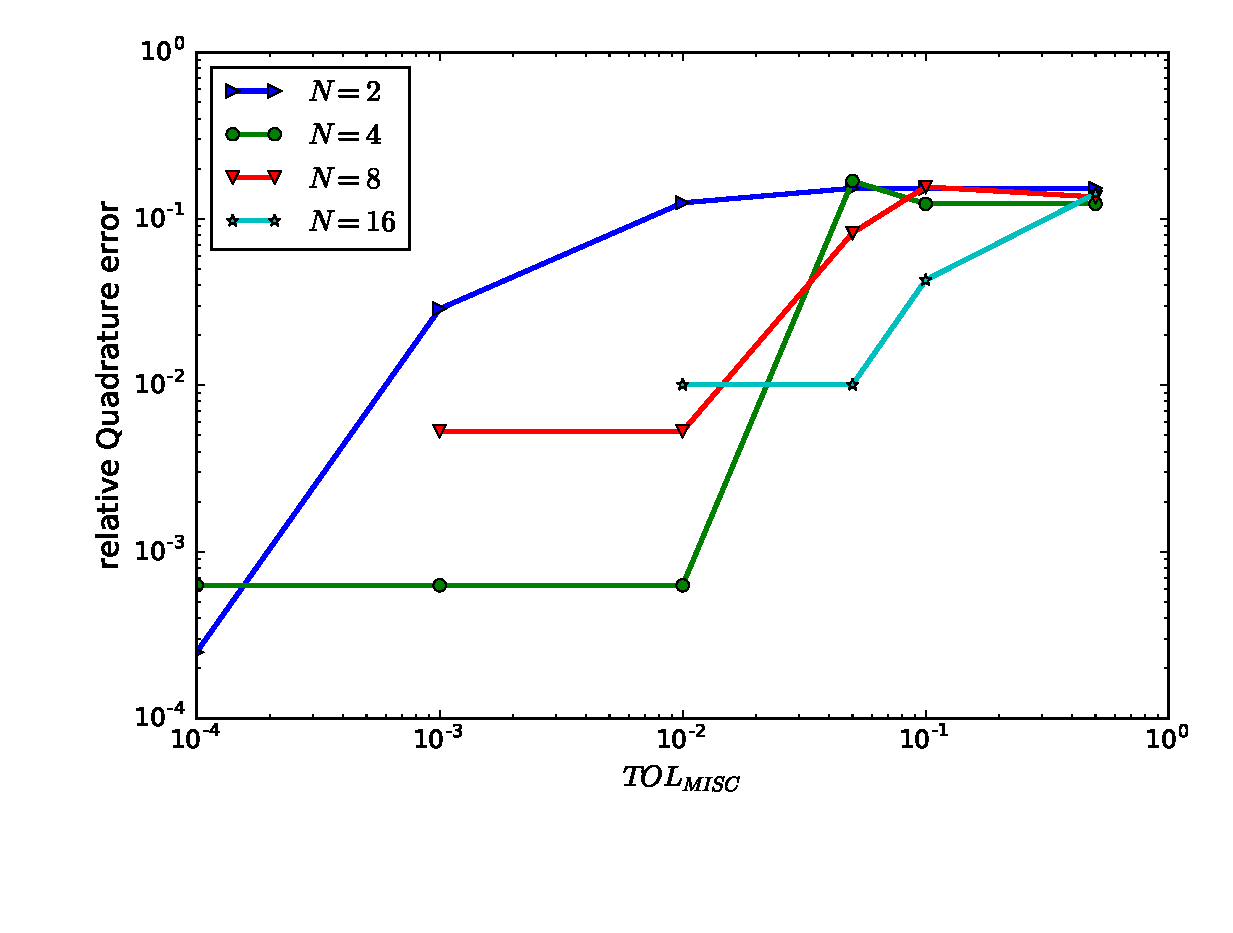
\includegraphics[width=0.4\linewidth]{./figures/rBergomi_MISC_quadratre_error/vs_TOL/set2/relative_quad_error_wrt_MISC_TOL_set2_non_rich_linear}
%	
%	
%	\caption{Quadrature error of MISC, without Richardson extrapolation, with different tolerances, to compute call option price for different number of time steps.}
%%	 See detailed values  in table \ref{Quadrature error of MISC to compute Call option price of the different tolerances for different number of time steps. Case  set $2$ parameters, without Richardson extrapolation. The numbers between parentheses are the corresponding absolute errors,linear}.}
%	\label{fig:Quadrature_error_set2_linear}
%\end{figure}





\FloatBarrier

\begin{table}[h!]
	\centering
	\begin{tabular}{l*{6}{c}r}
	\toprule[1.5pt]
	Method & & Steps  & &     \\
	\hline
		    & $2$ & $4$ & $8$  & $16$  \\
		\hline

		MISC ($\text{TOL}_{\text{MISC}}=10^{-1}$)  & $\underset{(0.54,0.15)}{\mathbf{
			0.69}}$& $ \underset{(0.29,0.13)}{\mathbf{    
			0.42}}$ & $ \underset{(0.15,0.16)}{\mathbf{     
			0.31
		}}$   & $ \underset{(0.07,0.04)}{\mathbf{     
			0.11
		}}$ \\

		MISC ($\text{TOL}_{\text{MISC}}=10^{-2}$)  & $\underset{(0.54,0.12)}{\mathbf{ 
			0.66}}$ & $ \underset{(0.29,6e-04)}{\mathbf{  0.29}}$ & $\underset{(0.15,0.01)}{\mathbf{    0.16}}$&  $ \underset{(0.07,0.01)}{\mathbf{0.08}}$  \\
%		MISC ($\text{TOL}_{\text{MISC}}=10^{-3}$)        & $\underset{(0.54,0.10)}{\mathbf{
%			0.64}}$  &  $ \underset{(0.29,6e-04)}{\mathbf{
%			0.29
%		}}$ &  $\underset{(0.15,0.01)}{\mathbf{    \red{0.16}}}$ &  $-$ \\
%		MISC ($\text{TOL}_{\text{MISC}}=10^{-4}$)        & $\underset{(0.54,3e-04)}{\mathbf{       0.54}}$  & $ \underset{(0.29,6e-04)}{\mathbf{
%			0.29
%		}}$  &  $-$ &  $-$\\
		%\hline
%		MC    & $\underset{(0.54,3e-03)}{\mathbf{0.54}}$  & $\underset{(0.29,1e-03)}{\mathbf{0.29}}$  &$\underset{(0.15,0.01)}{
%				\mathbf{0.16}}$ & \\	
%		M(\# MC samples)   & $8 \times 10^6$  & $8 \times 10^6$  &$10^5$ & \\	
				\hline
				MC    & $\underset{(0.54,0.51)}{\mathbf{1.05}}$  & $\underset{(0.295,0.295)}{\mathbf{0.59}}$  &$\underset{(0.155,0.155)}{
				\mathbf{0.31}}$& $\underset{(0.07,0.07)}{
				\mathbf{0.14}}$ \\	
		M(\# MC samples)   & $2 \times 10$  & $4 \times 10$  &$10^2$  & $4 \times 10^2$ \\
		\bottomrule[1.25pt]
	\end{tabular}
	\caption{Total relative error of MISC, without Richardson extrapolation, with different tolerances, and MC to compute the call option prices for different numbers of time steps. The values between parentheses correspond to the different errors contributing to the total relative error: for MISC we report the bias and quadrature errors and for MC we report the bias and the statistical errors estimates. The number of MC samples, $M$, is chosen to satisfy \eqref{optimal_number_samples}.}
	\label{Total error of MISC and MC to compute Call option price of the different tolerances for different number of time steps. Case $K=1$, $H=0.07$, without Richardson extrapolation. The numbers between parentheses are the corresponding absolute errors,linear}
\end{table}
\FloatBarrier




\begin{table}[htbp]
	\centering
	\begin{tabular}{l*{6}{c}r}
		\toprule[1.5pt]
	Method & & Steps  & &     \\
	\hline
	        & $2$ & $4$ & $8$  &$16$  \\
		\hline
%		MISC ($\text{TOL}_{\text{MISC}}=5.10^{-1}$)  & $0.08$ & $0.13$ & $0.2$ \\
		MISC ($\text{TOL}_{\text{MISC}}=10^{-1}$)  & $0.08$ & $0.13$ & $0.7$  & $163$ \\
%		MISC ($\text{TOL}_{\text{MISC}}=5.10^{-2}$)  & $0.08$ & $0.25$ & $7$   \\
		MISC ($\text{TOL}_{\text{MISC}}=10^{-2}$)  & $0.2$& $5$ & $333$ &  $1602$\\
%		MISC ($\text{TOL}_{\text{MISC}}=10^{-3}$)  &  $2$ & $73$ & $3650$ &  $-$ \\		
%		MISC ($\text{TOL}_{\text{MISC}}=10^{-4}$)  & $43$ & $1240$ & $-$ &   $-$\\	
%	
%		\hline
%		MC method & $220$  & $358$  & $9$ & \\
		\hline	
		MC method & $0.001$  & $0.003$  & $0.02$ & $0.2$ \\
		\bottomrule[1.25pt]	
%		Ratio of CPU time  $\left(\text{MC}/ \text{MISC} \right)$  &$\red{5}$ & $\red{   72 
%		}$  & $\red {  0.03	}$   \\
%		\hline
	\end{tabular}
	\caption{Comparison of the computational time (in seconds) of  MC and MISC, to compute the call option price of the rBergomi model for different numbers of time steps. The average MC CPU time is computed over $100$ runs.}
	\label{Comparsion of the computational time of  MC and MISC, used to compute Call option price of rBergomi model for different number of time steps. Case $K=1, H=0.07$, linear}
\end{table}
\FloatBarrier
%\subsubsection*{With Richardson extrapolation (level $1$)}

%\begin{table}[!h]
%	\centering
%	\begin{tabular}{l*{6}{c}r}
%		Method \textbackslash  Steps    &$1-2$         & $2-4$ & $4-8$ \\
%		\hline
%%		MISC ($\text{TOL}_{\text{MISC}}=5.10^{-1}$)  &$0.1260$ & $0.0756$ & $0.0687$\\
%		MISC ($\text{TOL}_{\text{MISC}}=10^{-1}$)  &$0.1260$ & $0.0756$ & $0.0702$   \\
%		MISC ($\text{TOL}_{\text{MISC}}=5.10^{-2}$)   &$0.1260$ & $0.0716$ & $0.0796$    \\
%		MISC ($\text{TOL}_{\text{MISC}}=10^{-2}$)  &$0.1456$ & $0.0838$ & $0.0796$  \\	
%		MISC ($\text{TOL}_{\text{MISC}}=10^{-3}$)  &$0.1497$ & $0.0838$ & $-$ \\
%		
%%		MISC ($\text{TOL}_{\text{MISC}}=10^{-4}$)  &$0.1501$ & $-$ & $-$ \\
%		\hline
%		MC method ($M=10^{6}$)   & $0.1552 $  & $0.0846 $  & $0.0804$  \\		
%		\hline
%	\end{tabular}
%	\caption{Call option price of the different methods for different number of time steps. Case set $2$ parameters of table \ref{table:Reference solution, using MC with $500$ time steps, of Call option price under rBergomi model, for different parameter constellation.}, using Richardson extrapolation (level $1$)}
%	\label{table:  Call option price of the different methods for different number of time steps. Case set $2$ parameter, using Richardson extrapolation (level $1$),linear}
%\end{table}

%\FloatBarrier
%
%\begin{table}[h!]
%	\centering
%	\begin{tabular}{l*{6}{c}r}
%		Method \textbackslash  Steps            & $1-2$ & $2-4$ & $4-8$  \\
%		\hline
%		MC Bias ($M=10^6$)  &$0.96$  & $0.07$  & $0.015$   \\	
%		
%		MC Statistical error ($M=10^6$)   & $1.3e-02$  & $4.1e-03$  & $2.1e-03$  \\	
%		\hline
%	\end{tabular}
%	\caption{Relative bias and statistical errors of MC, with Richardson extrapolation (level $1$), for computing call option price  for different number of time steps. The numbers between parentheses are the corresponding absolute errors.}
%	\label{Bias and Statistical errors of MC ($M=10^6$)  for computing Call option price  for different number of time steps. Case set $2$ parameters, with Richardson extrapolation (level1). The numbers between parentheses are the corresponding absolute errors.}
%\end{table}
%
%
%\FloatBarrier
%
%
%
%
%
%\begin{figure}[h!]
%	\centering
%	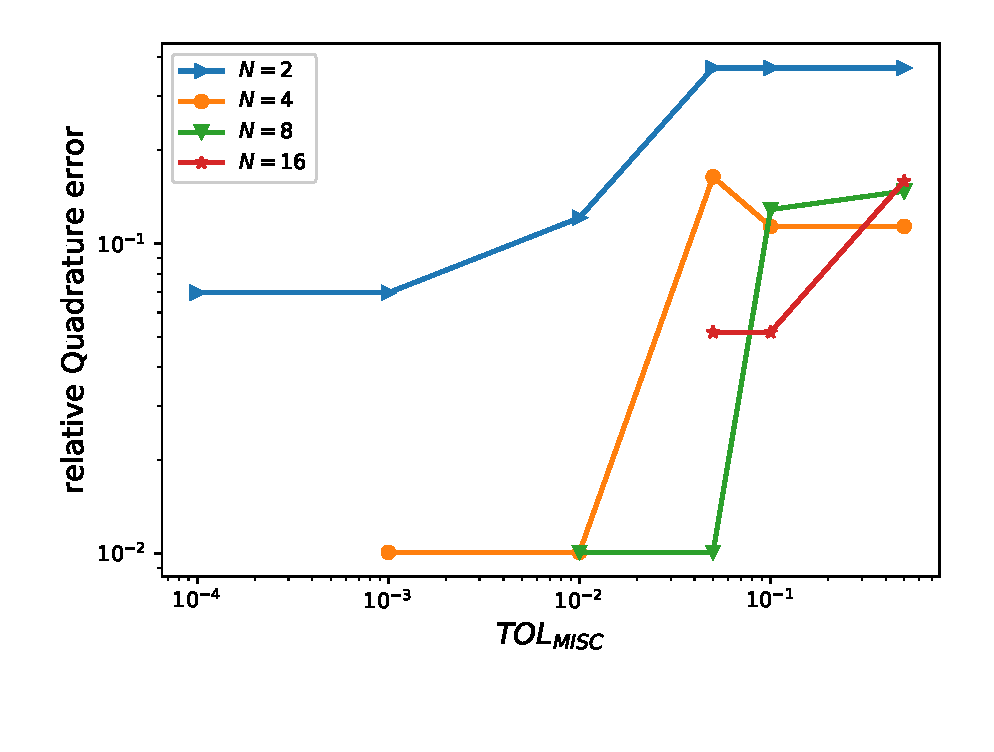
\includegraphics[width=0.4\linewidth]{./figures/rBergomi_MISC_quadratre_error/vs_TOL/set2/relative_quad_error_wrt_MISC_TOL_set2_with_rich_linear}
%	
%	
%	\caption{Quadrature error of MISC,with Richardson extrapolation (level $1$), with different tolerances,  to compute call option price for different number of time steps.}
	
%	  See detailed values  in table \ref{Quadrature error of MISC to compute Call option price of the different tolerances for different number of time steps. Case set $2$ parameters, with Richardson extrapolation(level $1$). The numbers between parentheses are the corresponding absolute errors,linear}.}
%	\label{fig:Quadrature_error_set2_linear_rich}
%\end{figure}


\begin{table}[h!]
	\centering
	\begin{tabular}{l*{6}{c}r}
		\toprule[1.5pt]
	Method & & Steps  & &     \\
	\hline
		          & $1-2$ & $2-4$ & $4-8$  \\
		\hline
		MISC ($\text{TOL}_{\text{MISC}}=10^{-1}$)  & $\underset{(0.96,0.37)}{\mathbf{  1.33}}$ & $\underset{(0.07,0.11)}{\mathbf{0.18}}$ & $\underset{(0.015,0.129)}{\mathbf{0.144}}$   \\
		MISC ($\text{TOL}_{\text{MISC}}=5.10^{-2}$)  & $\underset{(0.96,0.37)}{\mathbf{  1.33}}$ & $\underset{(0.07,0.16)}{\mathbf{ 0.23}}$ & $\underset{(0.015,0.010)}{\mathbf{  \red{0.025}}}$   \\
		MISC ($\text{TOL}_{\text{MISC}}=10^{-2}$)  & $\underset{(0.96,0.12)}{\mathbf{   1.08
		}}$ & $\underset{(0.07,0.01)}{\mathbf{0.08}}$ & $\underset{(0.015,0.010)}{\mathbf{ 0.025}}$  \\
%		MISC ($\text{TOL}_{\text{MISC}}=10^{-3}$)  & $\underset{(0.96,0.07)}{\mathbf{  1.03}}$ & $\underset{(0.07,0.01)}{\mathbf{    0.08}}$ & $\mathbf{-}$  \\
		

%		\hline
%		
%		MC &$\underset{(0.96,0.07)}{\mathbf{1.03}}$  & $\underset{(0.07,0.01)}{\mathbf{0.08}}$ & $\underset{(0.015,0.010)}{\mathbf{0.025}}$  \\
%		M(\# MC samples) & $3 \times 10^4$  & $2 \times 10^5$ & $4 \times 10^4$  \\
		
				\hline
		
		MC &$\underset{(0.96,0.92)}{\mathbf{1.88}}$  & $\underset{(0.07,0.07)}{\mathbf{0.14}}$ & $\underset{(0.015,0.015)}{\mathbf{\red{0.03}}}$  \\
		M(\# MC samples) & $10$  & $2 \times 10^3$ & $4 \times 10^4$  \\

		\bottomrule[1.25pt]
	\end{tabular}
	\caption{Total relative error of MISC, coupled with Richardson extrapolation (level $1$), with different tolerances,  and MC, coupled with Richardson extrapolation (level $1$), to compute the call option price  for different numbers of time steps. The values between parentheses correspond to the different errors contributing to the total relative error: for MISC we report the bias and quadrature errors and for MC we report the bias and the statistical errors. The number of MC samples, $M$, is chosen to satisfy \eqref{optimal_number_samples}. The values marked in red correspond to the values used for computational work comparison against MC method, reported in Table \ref{table:Summary of our numerical results.}.}
	\label{Total  error of MISC and MC to compute Call option price of the different tolerances for different number of time steps. Case set $2$ parameters, with Richardson extrapolation(level $1$). The numbers between parentheses are the corresponding absolute errors,relative}
\end{table}
\FloatBarrier


\begin{table}[h!]
	\centering
	\begin{tabular}{l*{6}{c}r}
		\toprule[1.5pt]
	Method & & Steps  & &     \\
	\hline
		          & $1-2$ & $2-4$ & $4-8$   \\
		\hline
%		MISC ($\text{TOL}_{\text{MISC}}=5.10^{-1}$)  & $0.1$ & $0.18$ & $0.3$   \\
		MISC ($\text{TOL}_{\text{MISC}}=10^{-1}$)  & $0.1$ & $0.2$ & $1.6$  \\
		MISC ($\text{TOL}_{\text{MISC}}=5.10^{-2}$)  & $0.1$ & $0.6$ & $\red{37}$  \\
		MISC ($\text{TOL}_{\text{MISC}}=10^{-2}$)  & $1.3$ & $6$ & $2382$  \\
%		MISC ($\text{TOL}_{\text{MISC}}=10^{-3}$)  & $3.5$ & $ 244$ & $-$   \\
		
%		MISC ($\text{TOL}_{\text{MISC}}=10^{-4}$)  & $140$ & $-$ & $-$ \\
%		\hline	
%		MC  &$\red{12}$ & $\red{113}$  & $\red{130}$   \\

			\hline	
		MC  &$0.003$ & $2$  & $\red{60}$   \\
		
%		\hline	
%		Ratio of CPU time $\left(\text{MC}/ \text{MISC} \right)$  &$\red{ 3.4
%		}$ & $\red{     18.8
%		}$  & $\red{ 3.5}
%		$  \\
		\bottomrule[1.25pt]
		\end{tabular}
		\caption{Comparison of the computational time (in seconds) of  MC and MISC, using Richardson extrapolation (level $1$), to compute the call option price of the rBergomi model for different numbers of time steps. The average MC CPU time is computed over $100$ runs. The values marked in red correspond to the values used for computational work comparison against MC method, reported in Table \ref{table:Summary of our numerical results.}.}
		\label{Comparsion of the computational time of  MC and MISC, using Richardson extrapolation (level $1$), used to compute Call option price of rBergomi model for different number of time steps. Case set $2$ parameters,linear}
		\end{table}
		
		\FloatBarrier
%	\subsubsection*{With Richardson extrapolation (level $2$)}
		
%
%		\begin{table}[h!]
%		\centering
%		\begin{tabular}{l*{6}{c}r}
%		Method \textbackslash  Steps           &$1-2-4$ & $2-4-8$ \\
%		\hline
%%		MISC ($\text{TOL}_{\text{MISC}}=5.10^{-1}$)& $0.0587$  & $0.0664 $ \\
%		
%		MISC ($\text{TOL}_{\text{MISC}}=10^{-1}$)  &$0.0587$  &$ 0.0702$   \\
%		MISC ($\text{TOL}_{\text{MISC}}=5.10^{-2}$)  & $0.0401$ & $0.0790$  \\
%		MISC ($\text{TOL}_{\text{MISC}}=10^{-2}$)  & $0.0623$ &  $0.0784$   \\
%%		MISC ($\text{TOL}_{\text{MISC}}=5.10^{-3}$)  & $0.0623$ & $-$   \\
%%		MISC ($\text{TOL}_{\text{MISC}}=10^{-3}$)  & $0.0608$ & $$  \\
%		
%		\hline
%		MC ($M=3.10^6$)  & $ 0.0601$ & $ 0.0787$   \\
%		\hline 
%	\end{tabular}
%	\caption{ Call option price of the different methods for different number of time steps. Case set $2$ parameters in tabel \ref{table:Reference solution, using MC with $500$ time steps, of Call option price under rBergomi model, for different parameter constellation.}, using Richardson extrapolation (level 2).}
%	\label{table: Call option price of the different methods for different number of time steps. Case $K=1,H=0.07$, using Richardson extrapolation_level2,linear}
%\end{table}




%\begin{table}[h!]
%	\centering
%	\begin{tabular}{l*{6}{c}r}
%		Method \textbackslash  Steps            & $1-2-4$ & $2-4-8$  \\
%		\hline
%		MC  Bias  ($M=3.10^6$)   &$ 0.24$  & $ 0.0058$   \\	
%		
%		MC Statistical error ($M=3.10^6$)   & $3.5e-03$  & $  1.8e-03$  \\	
%		
%		
%		
%		\hline
%	\end{tabular}
%	\caption{Relative bias and statistical errors of MC,  with Richardson extrapolation (level $2$), for computing call option price  for different number of time steps. The numbers between parentheses are the corresponding absolute errors.}
%	\label{Bias and Statistical errors of MC ($M=3.10^6$)  for computing Call option price  for different number of time steps. Case set $2$ parameters, with Richardson extrapolation (level2). The numbers between parentheses are the corresponding absolute errors.}
%\end{table}





\begin{table}[!h]
	\centering
	\begin{tabular}{l*{6}{c}r}
		\toprule[1.5pt]
	Method & & Steps  & &     \\
	\hline
		        & $1-2-4$ & $2-4-8$  \\
		\hline

		MISC ($\text{TOL}_{\text{MISC}}=10^{-1}$)  & $\underset{(0.24,0.30)}{\mathbf{ 0.54
		}}$ & $\underset{(0.006,0.107)}{\mathbf{ 0.113}}$ \\
		MISC ($\text{TOL}_{\text{MISC}}=5.10^{-2}$)  & $\underset{(0.24,0.25)}{\mathbf{   0.49
		}}$ & $\underset{(0.006,0.003)}{\mathbf{ \red{0.009}} }$  \\
		MISC ($\text{TOL}_{\text{MISC}}=10^{-2}$)  & $\underset{(0.24,0.03)}{\mathbf{ 0.27}}$ & $\underset{(0.006,0.003)}{\mathbf{ 0.009 }}$    \\	

%		\hline
%		MC   & $\underset{(0.24,0.03)}{\mathbf{0.27}}$  & $\underset{(0.006,0.003)}{\mathbf{0.009}}$    \\
%			M(\# MC samples) & $5 \times 10^4$  & $7 \times 10^5$   \\
			
				\hline
		MC   & $\underset{(0.24,0.21)}{\mathbf{0.45}}$  & $\underset{(0.006,0.006)}{\mathbf{\red{0.012}}}$    \\
			M(\# MC samples) & $4 \times 10^2$  & $4 \times 10^5$   \\
		\bottomrule[1.25pt]
	\end{tabular}
	\caption{Total relative  error of MISC, coupled with Richardson extrapolation (level $2$), with different tolerances, and MC, coupled with Richardson extrapolation (level $2$), to compute the call option price for different numbers of time steps.  The values between parentheses correspond to the different errors contributing to the total relative error: for MISC we report the bias and quadrature errors and for MC we report the bias and the statistical errors. The number of MC samples, $M$, is chosen to satisfy \eqref{optimal_number_samples}. The values marked in red correspond to the values used for computational work comparison against MC method, reported in Table \ref{table:Summary of our numerical results.}.}
	\label{Total  error of MISC and MC to compute Call option price of the different tolerances for different number of time steps. Case set $2$ parameters, with Richardson extrapolation(level $2$). The numbers between parentheses are the corresponding absolute errors,linear}
\end{table}
\FloatBarrier

\begin{table}[!h]
	\centering
	\begin{tabular}{l*{6}{c}r}
		\toprule[1.5pt]
	Method & & Steps  & &     \\
	\hline
		           & $1-2-4$ & $2-4-8$   \\
		\hline

		MISC ($\text{TOL}_{\text{MISC}}=10^{-1}$)  & $0.2$ & $2$ &   \\
		MISC ($\text{TOL}_{\text{MISC}}=5.10^{-2}$)  & $0.5$ & $\red{74}$  \\
		MISC ($\text{TOL}_{\text{MISC}}=10^{-2}$)  & $9$ & $3455$   \\
%		MISC ($\text{TOL}_{\text{MISC}}=5.10^{-3}$)  & $30$ & $-$  \\	
%		MISC ($\text{TOL}_{\text{MISC}}=10^{-3}$)  & $693$ & $-$  \\	
%		\hline
%		MC    & $ \red{  118}$  & $\red{1274}$  \\
%		
		\hline
		MC    & $ 0.2$  & $\red{690}$  \\
		
%		\hline
%		Ratio of CPU time $\left(\text{MC}/ \text{MISC} \right)$  &$\red{13}$ & $\red{  17}$   \\
		\bottomrule[1.25pt]
	\end{tabular}
	\caption{Comparison of the computational time (in seconds) of  MC and MISC, using Richardson extrapolation (level $2$), to compute the call option price of the rBergomi model for different numbers of time steps. The 	average MC CPU time is computed over $100$ runs. The values marked in red correspond to the values used for computational work comparison against MC method, reported in Table \ref{table:Summary of our numerical results.}.}
	\label{Comparsion of the computational time of  MC and MISC, using Richardson extrapolation (level $2$), used to compute Call option price of rBergomi model for different number of time steps. Case set $2$ parameters,linear}
\end{table}

\FloatBarrier

\begin{figure}[h!]
	\centering
	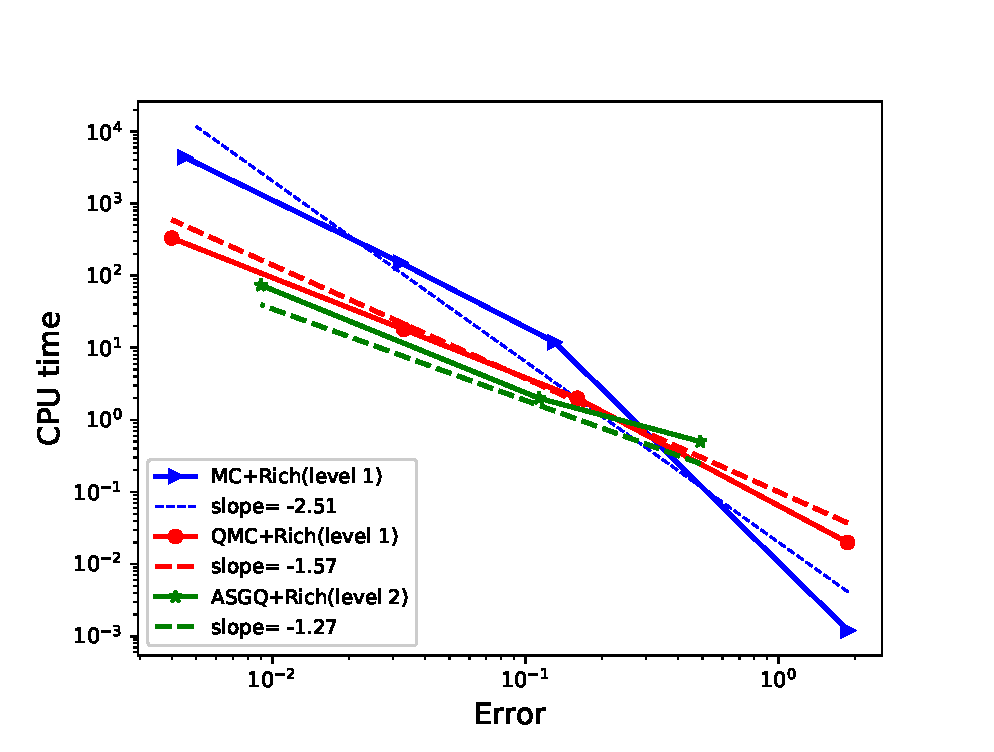
\includegraphics[width=0.6\linewidth]{./figures/rBergomi_Complexity_rates/set2/error_vs_time_set2_full_comparison}
	
	\caption{Computational work comparison for  MISC and MC methods (with and without) Richardson extrapolation, for the case of parameter set $1$ in Table \ref{table:Reference solution, using MC with $500$ time steps, of Call option price under rBergomi model, for different parameter constellation.}. This plot shows that to achieve a relative error below $1\%$, MISC coupled with level $2$ of Richardson extrapolation is the best option in terms of computational time. Furthermore, applying Richardson extrapolation brings a significant improvement for MISC and MC methods, in terms of numerical complexity.}
	\label{fig:Complexity plot for  MISC for Case set $2$ parameters, comparison}
\end{figure}




\FloatBarrier

\subsubsection{Case of parameters in Set 2, in Table \ref{table:Reference solution, using MC with $500$ time steps, of Call option price under rBergomi model, for different parameter constellation.} }\label{sec:Case of set 3 parameters}

In this section, we only conduct our numerical experiments for the case without Richardson extrapolation, since the results show that we meet a small enough error tolerance without the need to apply   Richardson extrapolation. Our numerical experiments show that MISC requires  approximately $20\%$ of the work of MC method, to achieve  a total relative error of around $0.2\%$ (see Figure \ref{fig:Complexity plot for  MISC for case set $3$ parameters, comparison} and  Tables \ref{Comparsion of the computational time of  MC and MISC, used to compute Call option price of rBergomi model for different number of time steps. Case set3} and \ref{Total error of MISC and MC to compute Call option price of the different tolerances for different number of time steps. Case set 3, without Richardson extrapolation. The numbers between parentheses are the corresponding absolute errors.}).  

%\subsubsection*{Without Richardson extrapolation}

%\begin{table}[h!]
%	\centering
%	\begin{tabular}{l*{6}{c}r}
%		Method \textbackslash  Steps            & $2$ & $4$ & $8$ & $16$ &   \\
%		\hline
%%		MISC ($\text{TOL}_{\text{MISC}}=5.10^{-1}$)  & $0.1258$ & $0.1239$ & $0.1231$ & $0.1227$  \\
%		MISC ($\text{TOL}_{\text{MISC}}=10^{-1}$)  & $0.1258$ & $0.1239$ & $0.1231$ & $0.1229$  \\
%%		MISC ($\text{TOL}_{\text{MISC}}=5.10^{-2}$)  & $0.1258$ & $0.1239$ & $0.1231$ & $0.1241$  \\
%		MISC ($\text{TOL}_{\text{MISC}}=10^{-2}$)  & $0.1258$ & $0.1246$ & $0.1248$ & $0.1250$  \\
%		
%		MISC ($\text{TOL}_{\text{MISC}}=10^{-3}$)  & $0.1271$ & $0.1259$ & $0.1252$ & $0.1249$  \\
%		MISC ($\text{TOL}_{\text{MISC}}=10^{-4}$)  & $0.1270$ & $0.1258$ & $0.1252$ & $-$  \\
%		
%%			MISC ($\text{TOL}_{\text{MISC}}=10^{-5}$)  & $0.1270$ &$0.1258$ &  $0.1252$ & $-$  \\
%		\hline
%		MC method ($M=3.10^{6}$)   & $    0.1269$ & $0.1257$  & $0.1253$ & $0.1249$ \\		
%		
%		\hline
%	\end{tabular}
%	\caption{ Call option price of the different methods for different number of time steps. Case of set $3$ parameters in table \ref{table:Reference solution, using MC with $500$ time steps, of Call option price under rBergomi model, for different parameter constellation.}, without Richardson extrapolation.}
%	\label{table: Call option price of the different methods for different number of time steps. Case set 3}
%\end{table}

%\FloatBarrier 
%
%\begin{table}[h!]
%	\centering
%	\begin{tabular}{l*{6}{c}r}
%		Method \textbackslash  Steps            & $2$ & $4$ & $8$ & $16$  \\
%		\hline
%		MC Bias ($M=3.10^6$)   & 	$ \underset{(    0.0022)}{\mathbf{0.0174}}$  & $\underset{(0.001)}{\mathbf{0.0078}}$  & $\underset{(0.0005)}{\mathbf{0.0042}}$ & $\underset{(0.0001)}{\mathbf{0.0008}}$\\ 
%		
%		MC Statistical error ($M=3.10^6$)  &  $\underset{(   6.2e-05)} {\mathbf{5.0e-04}}$  & $\underset{(5.9e-05)} {\mathbf{4.7e-04}}$  & $\underset{(5.8e-05)} {\mathbf{4.6e-04 }}$ & $\underset{(5.8e-05)} {\mathbf{4.6e-04 }}$	\\
%		
%		\hline
%	\end{tabular}
%	\caption{Bias and statistical errors of MC   for computing call option price  for different number of time steps. Case set $2$, without Richardson extrapolation. The numbers between parentheses are the corresponding absolute errors.}
%	\label{Bias and Statistical errors of MC ($M=10^6$)  for computing Call option price  for different number of time steps. Case set 3, without Richardson extrapolation. The numbers between parentheses are the corresponding absolute errors.}
%\end{table}
%
%
%
%
%\FloatBarrier
%
%	\begin{figure}[h!]
%		\centering
%		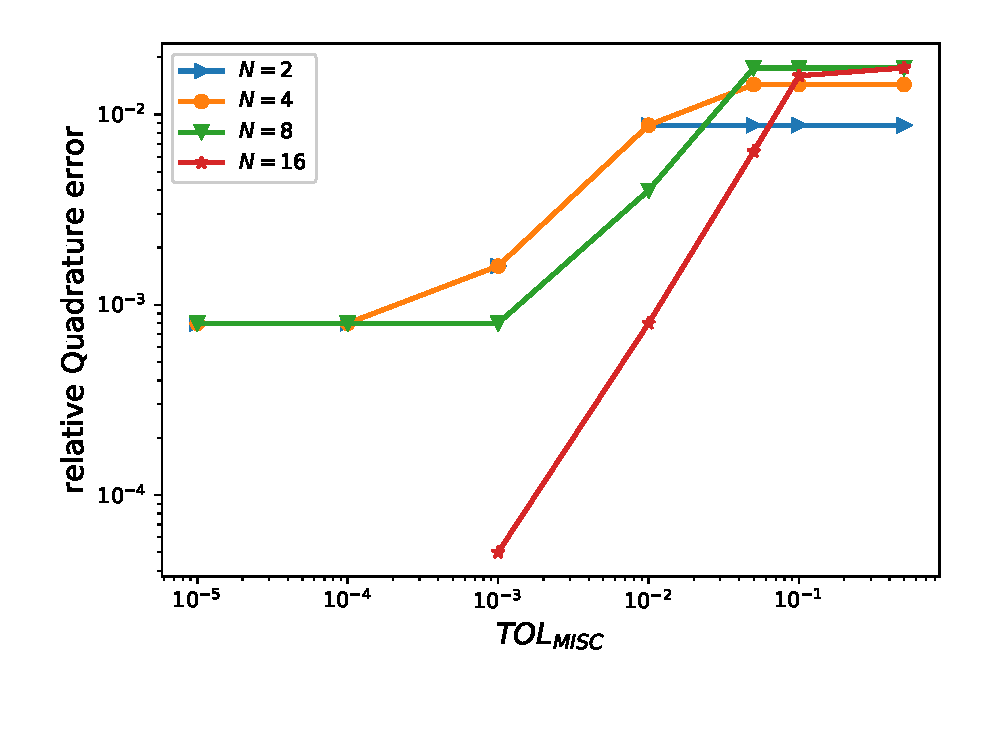
\includegraphics[width=0.35\linewidth]{./figures/rBergomi_MISC_quadratre_error/vs_TOL/set5/relative_quad_error_wrt_MISC_TOL_set5_non_rich}
%	
%	
%	\caption{Quadrature error of MISC, with different tolerances, to compute call option price  for different number of time steps. Case  set $2$ parameters, without Richardson extrapolation. }
%%	 See detailed values  in table \ref{Quadrature error of MISC to compute Call option price of the different tolerances for different number of time steps. Case  set $3$ parameters, without Richardson extrapolation. The numbers between parentheses are the corresponding absolute errors.}.}
%	\label{fig:Quadrature_error_set3}
%\end{figure}
%
\FloatBarrier




\begin{table}[h!]
	\centering
	\begin{tabular}{l*{6}{c}r}
	\toprule[1.5pt]
	Method & & Steps  & &     \\
	\hline		
		         & $2$ & $4$ & $8$ & $16$  \\
		\hline
%%
		MISC ($\text{TOL}_{\text{MISC}}=10^{-1}$)  &  $\underset{(0.02,0.01)}{\mathbf{0.03}}$ & $\underset{(0.008,0.014)}{\mathbf{0.022}}$& $\underset{(0.004,0.018)}{\mathbf{ 0.022}}$ & $\underset{(0.001,0.016)}{\mathbf{ 0.017}}$   \\

		MISC ($\text{TOL}_{\text{MISC}}=10^{-2}$)  &  $\underset{(0.02,0.01)}{\mathbf{0.03}}$ & $\underset{(0.008,0.009)}{\mathbf{0.017}}$& $\underset{(0.004,0.004)}{\mathbf{ 0.008}}$ & $\underset{(0.001,4e-04)}{\mathbf{ \red{0.001}}}$  \\
		MISC ($\text{TOL}_{\text{MISC}}=10^{-3}$)  &  $\underset{(0.02,8e-04)}{\mathbf{0.02}}$ & $\underset{(0.008,8e-04)}{\mathbf{0.009}}$& $\underset{(0.004,8e-04)}{\mathbf{0.005}}$  & $\underset{(0.001,4e-04)}{\mathbf{ 0.001}}$  \\
%%%		MISC ($\text{TOL}_{\text{MISC}}=10^{-4}$)  &  $\underset{(0.02,8e-04)}{\mathbf{\red{0.02}}}$ & $\underset{(0.008,8e-04)}{\mathbf{\red{0.009}}}$& $\underset{(0.004,8e-04)}{\mathbf{0.005}}$ & $\mathbf{ -}$ \\
%%
%%		%\hline
%%%		MC    & $\underset{(0.02,5e-04)}{\mathbf{0.02}}$  &  $\underset{(0.008,5e-04)}{\mathbf{0.009}}$  & $\underset{(0.004,5e-04)}{\mathbf{0.005}}$ & $\underset{(0.001,4e-04)}{\mathbf{0.001}}$  \\	
%%%			M(\# MC samples) 	& $5 \times 10^6$  &  $5 \times 10^6$  & $5 \times 10^6$ & $5 \times 10^6$  \\
			\hline
				MC    & $\underset{(0.02,0.02)}{\mathbf{0.04}}$  &  $\underset{(0.008,0.008)}{\mathbf{0.016}}$  & $\underset{(0.004,0.003)}{\mathbf{0.007}}$ & $\underset{(0.001,0.001)}{\mathbf{\red{0.002}}}$  \\	
			M(\# MC samples) 	& $4 \times 10^3$  &  $2 \times 10^4$  & $  10^5$ & $10^6$  \\
		\bottomrule[1.25pt]
	\end{tabular}
	\caption{Total relative error of MISC, without Richardson extrapolation,  with different tolerances, and MC to compute the call option price for different numbers of time steps. The values between parentheses correspond to the different errors contributing to the total relative error: for MISC we report the bias and quadrature errors and for MC we report the bias and the statistical errors estimates. The number of MC samples, $M$, is chosen to satisfy \eqref{optimal_number_samples}. The values marked in red correspond to the values used for computational work comparison against MC method, reported in Table \ref{table:Summary of our numerical results.}.}
	\label{Total error of MISC and MC to compute Call option price of the different tolerances for different number of time steps. Case set 3, without Richardson extrapolation. The numbers between parentheses are the corresponding absolute errors.}
\end{table}


\FloatBarrier
\begin{table}[h!]
	\centering
	\begin{tabular}{l*{6}{c}r}
	\toprule[1.5pt]
	Method & & Steps  & &     \\
	\hline	
         & $2$ & $4$ & $8$ & $16$ &   \\
		\hline
%		MISC ($\text{TOL}_{\text{MISC}}=5.10^{-1}$)  & $0.1$ & $0.1$ & $0.2$ & $0.4$  \\
		MISC ($\text{TOL}_{\text{MISC}}=10^{-1}$)  & $0.1$ & $0.1$ & $0.2$ & $0.8$ \\
%		MISC ($\text{TOL}_{\text{MISC}}=5.10^{-2}$)  & $0.1$ & $0.1$ & $0.2$ & $22$  \\
		MISC ($\text{TOL}_{\text{MISC}}=10^{-2}$)  & $0.1$ & $0.5$ & $8$ & $\red{92}$ \\
		MISC ($\text{TOL}_{\text{MISC}}=10^{-3}$)  & $0.5$ & $3$ & $24$ & $226$ \\
%		MISC ($\text{TOL}_{\text{MISC}}=10^{-4}$)  & $\red{1}$ & $\red{6}$ & $80$ & $-$\\
%		MISC ($\text{TOL}_{\text{MISC}}=10^{-5}$)  & $2$ & $32$ & $1760$ & $-$
%		 \\
%		\hline
%		MC method   & $ \red{122}
%		
%		$  & $  \red{260}$  & $  \red{427}$ & $ \red{766}
%		$  \\	
		\hline
		MC method   & $ 0.15
		
		$  & $  1.6$  & $  16.5$ & $ \red{494}
		$  \\	
%		\hline
%		Ratio of CPU time  $\left(MC/MISC \right)$ & $ \red{244}
%		
%		$  & $  \red{86}$  & $  \red{  18
%		}$ & $ \red{ 8}
%		$  \\	
		
		\bottomrule[1.25pt]
	\end{tabular}
	\caption{Comparison of the computational time (in seconds) of  MC and MISC, to compute the call option price of the rBergomi model for different numbers of time steps. The average  MC CPU time is computed over $100$ runs. The values marked in red correspond to the values used for computational work comparison against MC method, reported in Table \ref{table:Summary of our numerical results.}. }
	\label{Comparsion of the computational time of  MC and MISC, used to compute Call option price of rBergomi model for different number of time steps. Case set3}
\end{table}
%\FloatBarrier
%	\begin{figure}[h!]
%	\centering
%	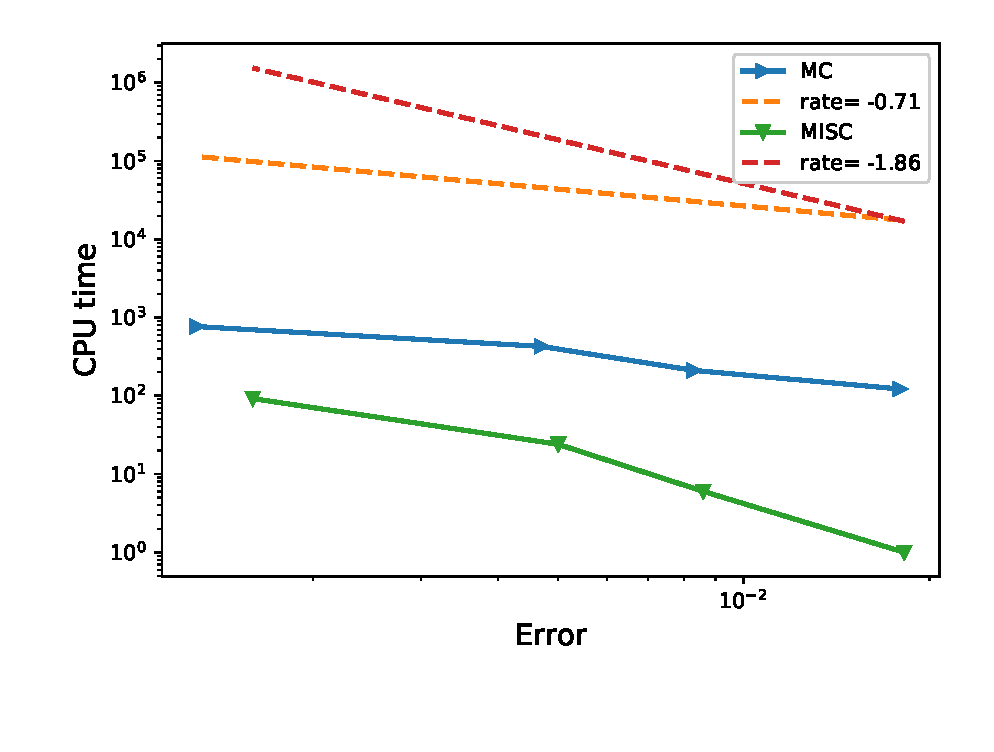
\includegraphics[width=0.5\linewidth]{./figures/rBergomi_Complexity_rates/set5/error_vs_time_set5}
%
%	\caption{Comparison of computational work  for MC and MISC, without Richardson extrapolation.}
%	\label{fig:Complexity plot for MC and MISC for Case set $3$ parameters}
%\end{figure}



\FloatBarrier

%\subsubsection*{With Richardson extrapolation (level $1$)}
%\FloatBarrier
%\begin{table}[h!]
%	\centering
%	\begin{tabular}{l*{6}{c}r}
%		Method \textbackslash  Steps    &$1-2$         & $2-4$ & $4-8$ & $8-16$\\
%		\hline
%%		MISC ($\text{TOL}_{\text{MISC}}=5.10^{-1}$)   &$ 0.1261$ & $0.1220$ & $0.1222$ & $0.1223$\\
%		MISC ($\text{TOL}_{\text{MISC}}=10^{-1}$)   &$ 0.1261$ & $0.1220$  &$0.1222$ & $0.1226$\\
%%		MISC ($\text{TOL}_{\text{MISC}}=5.10^{-2}$)   &$ 0.1261$ & $0.1220$  & $0.1222$ & $0.1240$ \\
%		MISC ($\text{TOL}_{\text{MISC}}=10^{-2}$)   &$ 0.1267$ & $0.1230$ & $0.1245$ & $0.1247$  \\	
%		MISC ($\text{TOL}_{\text{MISC}}=10^{-3}$)   &$0.1285$ & $0.1247$ & $0.1247$ &  $0.1247$ \\
%%		MISC ($\text{TOL}_{\text{MISC}}=10^{-4}$)  &$0.1285$ & $0.1247$ & $0.1247$ & $-$ \\
%%			MISC ($\text{TOL}_{\text{MISC}}=10^{-5}$)  &$0.1285$ & $0.1247$ &  $0.1247$ & $-$ \\
%	
%		\hline
%		MC method ($M=10^{7}$)   & $     0.1284$  & $ 
%		0.1251$  & $0.1249$ & $  0.1248$ \\		
%		\hline
%	\end{tabular}
%	\caption{Call option price of the different methods for different number of time steps. Case set $3$ parameters of table \ref{table:Reference solution, using MC with $500$ time steps, of Call option price under rBergomi model, for different parameter constellation.}, using Richardson extrapolation (level $1$).}
%	\label{table:  Call option price of the different methods for different number of time steps. Case set $5$ parameter, using Richardson extrapolation (level $3$)}
%\end{table}
%\FloatBarrier
%
%
%\begin{table}[h!]
%	\centering
%	\begin{tabular}{l*{6}{c}r}
%		Method \textbackslash  Steps            & $1-2$ & $2-4$ & $4-8$ & $8-16$  \\
%		\hline
%		MC Bias ($M=10^7$)  &$\underset{(  0.0037
%			)}{\mathbf{0.0295}}$  & $\underset{( 0.0003)}{\mathbf{0.0025}}$  & $\underset{(   0.0001)}{\mathbf{0.0009}}$  & $\underset{(  6.2e-05)}{\mathbf{0.0005}}$ \\	
%		
%		MC Statistical error ($M=10^7$)   & $\underset{(  4.4e-05)}{\mathbf{3.5e-04}}$  & $\underset{(   4.2e-05)}{\mathbf{3.4e-04}}$  & $\underset{(  4.1e-05)}{\mathbf{3.3e-04}}$ & $\underset{(  4.1e-05)}{\mathbf{3.3e-04}}$ \\	
%	
%		\hline
%	\end{tabular}
%	\caption{Bias and statistical errors of MC   for computing call option price  for different number of time steps. Case set $2$ parameters in table \ref{table:Reference solution, using MC with $500$ time steps, of Call option price under rBergomi model, for different parameter constellation.}, with Richardson extrapolation (level $1$). The numbers between parentheses are the corresponding absolute errors.}
%	\label{Bias and Statistical errors of MC ($M=10^7$)  for computing Call option price  for different number of time steps. Case set $3$ parameters, with Richardson extrapolation (level1). The numbers between parentheses are the corresponding absolute errors.}
%\end{table}
%
%
%
%\FloatBarrier
%
%
%
%
%\begin{figure}[h!]
%	\centering
%	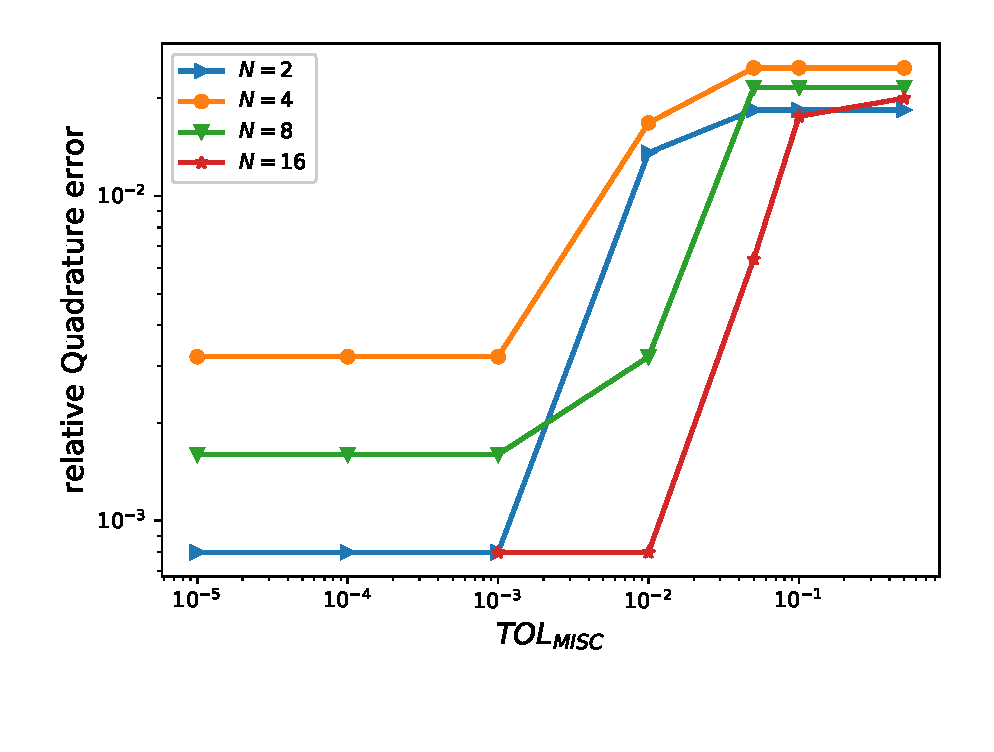
\includegraphics[width=0.35\linewidth]{./figures/rBergomi_MISC_quadratre_error/vs_TOL/set5/relative_quad_error_wrt_MISC_TOL_set5_with_rich}
%	
%	
%	\caption{Quadrature error of MISC, with  different tolerances,  to compute call option price, for different number of time steps. Case  set $2$ parameters, with Richardson extrapolation.}
%%	  See detailed values  in table \ref{Quadrature error of MISC to compute Call option price of the different tolerances for different number of time steps. Case set $3$ parameters, with Richardson extrapolation(level $1$). The numbers between parentheses are the corresponding absolute errors.}.}
%	\label{fig:Quadrature_error_set3_rich}
%\end{figure}




%\FloatBarrier
%\begin{table}[h!]
%	\centering
%	\begin{tabular}{l*{6}{c}r}
%		Method \textbackslash  Steps           & $2-4$ & $4-8$ & $8-16$  \\
%		\hline
%
%		MISC ($\text{TOL}_{\text{MISC}}=10^{-1}$)  &$\underset{(0.003,0.024)}{\mathbf{0.027}}$  &$\underset{(0.001,0.022)}{\mathbf{0.023}}$ & $\underset{(0.001,0.017)} {\mathbf{0.018}}$  \\
%
%			MISC ($\text{TOL}_{\text{MISC}}=10^{-2}$)  & $\underset{(0.003,0.016)}{\mathbf{0.019}}$  & $\underset{(0.001,0.003)}{\mathbf{0.004}}$ & $\underset{(0.001,0.001)} {\mathbf{\red{0.002}}}$  \\
%		MISC ($\text{TOL}_{\text{MISC}}=10^{-3}$)  & $\underset{(0.003,0.003)}{\mathbf{\red{0.006}}}$  & $\underset{(0.001,0.002)}{\mathbf{\red{0.003}}}$ & $\underset{(0.001,0.001)} {\mathbf{0.002}}$  \\
%	
%	\hline
%
%		MC    & $\underset{(0.003,0.003)}{\mathbf{0.006}}$  &   $\underset{(0.001,0.002)}{\mathbf{0.003}}$  &  $\underset{(0.001,0.001)}{\mathbf{0.002}}$  \\
%			M(\# MC samples) & $5 \times 10^4$  &   $4 \times 10^5$  &  $2 \times 10^6$  \\
%		\hline
%	\end{tabular}
%	\caption{Total relative error of MISC, coupled with Richardson extrapolation (level $1$), with different tolerances, and MC, coupled with Richardson extrapolation (level $1$), to compute call option price  for different number of time steps.}
%	\label{Total  error of MISC and MC to compute Call option price of the different tolerances for different number of time steps. Case set $3$ parameters, with Richardson extrapolation(level $1$). The numbers between parentheses are the corresponding absolute errors.}
%\end{table}
%
%\FloatBarrier
%
%\begin{table}[h!]
%	\centering
%	\begin{tabular}{l*{6}{c}r}
%		Method \textbackslash  Steps            & $2-4$ & $4-8$ & $8-16$ &   \\
%		\hline
%%		MISC ($\text{TOL}_{\text{MISC}}=5.10^{-1}$)    & $0.15$ & $0.25$ & $0.5$  \\
%		MISC ($\text{TOL}_{\text{MISC}}=10^{-1}$)   & $0.15$ & $0.25$ & $1$  \\
%%		MISC ($\text{TOL}_{\text{MISC}}=5.10^{-2}$)    &  $0.15$ & $0.25$ & $12.5$  \\
%		MISC ($\text{TOL}_{\text{MISC}}=10^{-2}$)   & $0.6$ & $10$ & $\red{112}$  \\
%		MISC ($\text{TOL}_{\text{MISC}}=10^{-3}$)  & $\red{3.5}$ & $\red{34}$ & $3150$ \\
%%		MISC ($\text{TOL}_{\text{MISC}}=10^{-4}$) & $11$ & $328$ & $-$  \\
%%		MISC ($\text{TOL}_{\text{MISC}}=10^{-5}$)   & $39$ & $2160$ & $-$  \\
%		\hline	
%			MC  & $45$  & $438$  & $2240$ \\
%			
%%			\hline
%%				Ratio of CPU time  $\left(\text{MC}/ \text{MISC} \right)$   & $13$  & $13$  & $20$ \\
%
%		\hline
%	\end{tabular}
%	\caption{Comparison of the computational time (in Seconds) of  MC and MISC, using Richardson extrapolation (level $1$), used to compute call option price of the rBergomi model for different number of time steps. The
%average MC CPU time is computed over $100$ runs.}
%	\label{Comparsion of the computational time of  MC and MISC, using Richardson extrapolation (level $1$), used to compute Call option price of rBergomi model for different number of time steps. Case set $3$ parameters}
%\end{table}

\FloatBarrier


	\begin{figure}[h!]
	\centering
	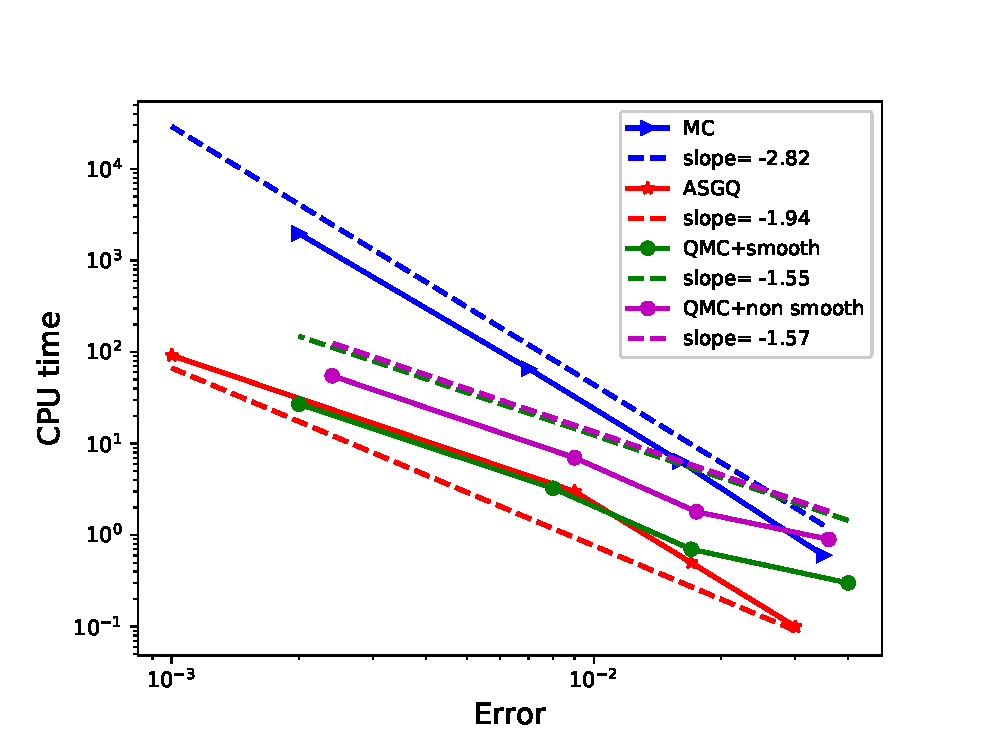
\includegraphics[width=0.5\linewidth]{./figures/rBergomi_Complexity_rates/set5/error_vs_time_set5_full_comparison}
	
	\caption{Computational work comparison for  MISC  and MC methods, for the case of parameter set $2$ in Table \ref{table:Reference solution, using MC with $500$ time steps, of Call option price under rBergomi model, for different parameter constellation.}. This plot shows that to achieve a relative error below $1\%$, MISC outperforms MC method in terms of computational time.}
	\label{fig:Complexity plot for  MISC for case set $3$ parameters, comparison}
\end{figure}


\FloatBarrier
\subsubsection{Case of parameters in Set 3, in Table \ref{table:Reference solution, using MC with $500$ time steps, of Call option price under rBergomi model, for different parameter constellation.} }\label{sec:Case of set 4 parameters}


In this section, we only conduct our numerical experiments for the case without Richardson extrapolation, since the results show that we meet a small enough error tolerance without the need to apply   Richardson extrapolation.  Our numerical experiments show that MISC requires  approximately $14\%$ of the work of MC method, to achieve a total relative error of around $0.4\%$ (see Figure \ref{fig:Complexity plot for MC and MISC for case set $4$ parameters} and Tables \ref{Comparsion of the computational time of  MC and MISC, used to compute Call option price of rBergomi model for different number of time steps. Case set4} and \ref{Total error of MISC and MC to compute Call option price of the different tolerances for different number of time steps. Case set 4, without Richardson extrapolation. The numbers between parentheses are the corresponding absolute errors.}). 

%\FloatBarrier
%\begin{table}[h!]
%	\centering
%	\begin{tabular}{l*{6}{c}r}
%		Method \textbackslash  Steps            & $2$ & $4$ & $8$ & $16$ &   \\
%		\hline
%%		MISC ($\text{TOL}_{\text{MISC}}=5.10^{-1}$)  & $0.2413$ & $0.2403$ & $0.2403$ & $0.2396$  \\
%		MISC ($\text{TOL}_{\text{MISC}}=10^{-1}$)  & $0.2413$ &$0.2403$& $0.2403$ & $0.2397$   \\
%%		MISC ($\text{TOL}_{\text{MISC}}=5.10^{-2}$)  &$0.2413$ & $0.2403$ & $0.2403$ & $0.2406$  \\
%		MISC ($\text{TOL}_{\text{MISC}}=10^{-2}$)  &$0.2413$ & $0.2403$ & $0.2409$ & $0.2413$  \\
%		
%		MISC ($\text{TOL}_{\text{MISC}}=10^{-3}$)  & $0.2413$ & $0.2411$ & $0.2414$ & $0.2413$  \\
%		MISC ($\text{TOL}_{\text{MISC}}=10^{-4}$)  &  $0.2421$ & $0.2416$ & $0.2414$ & $-$  \\
%		
%%		MISC ($\text{TOL}_{\text{MISC}}=10^{-5}$)  & $0.2421$ &$0.2416$ &  $0.2414$ & $-$  \\
%		\hline
%		MC method ($M=5.10^{6}$)   & $0.2420$ & $0.2416$  & $0.2414$ & $0.2413$ \\		
%		
%		\hline
%	\end{tabular}
%	\caption{ Call option price of the different methods for different number of time steps. Case set $4$ parameters in table \ref{table:Reference solution, using MC with $500$ time steps, of Call option price under rBergomi model, for different parameter constellation.}, without Richardson extrapolation.}
%	\label{table: Call option price of the different methods for different number of time steps. Case set 4}
%\end{table}
%\FloatBarrier
%
%\begin{table}[h!]
%	\centering
%	\begin{tabular}{l*{6}{c}r}
%		Method \textbackslash  Steps            & $2$ & $4$ & $8$ & $16$  \\
%		\hline
%		MC Bias ($M=5.10^6$)   & 	$ \underset{(    0.0013)}{\mathbf{0.0054}}$  & $\underset{(0.0008)}{\mathbf{0.0035
%		}}$  & $\underset{(0.0007)}{\mathbf{0.0029}}$ & $\underset{(0.0006)}{\mathbf{0.0024}}$\\ 
%		
%		MC Statistical error ($M=5.10^6$)  &  $\underset{(   8.3e-05)} {\mathbf{3.4e-04}}$  & $\underset{(8.1e-05)} {\mathbf{3.4e-04}}$  & $\underset{(8.0e-05)} {\mathbf{3.3e-04 }}$ & $\underset{(8.0e-05)} {\mathbf{3.3e-04}}$	\\
%		
%		\hline
%	\end{tabular}
%	\caption{Bias and statistical errors of MC   for computing call option price  for different number of time steps. Case set $3$, without Richardson extrapolation. The numbers between parentheses are the corresponding absolute errors.}
%	\label{Bias and Statistical errors of MC ($M=5.10^6$)  for computing Call option price  for different number of time steps. Case set 4, without Richardson extrapolation. The numbers between parentheses are the corresponding absolute errors.}
%\end{table}
%
%
%\FloatBarrier
%
%
%\begin{figure}[h!]
%	\centering
%	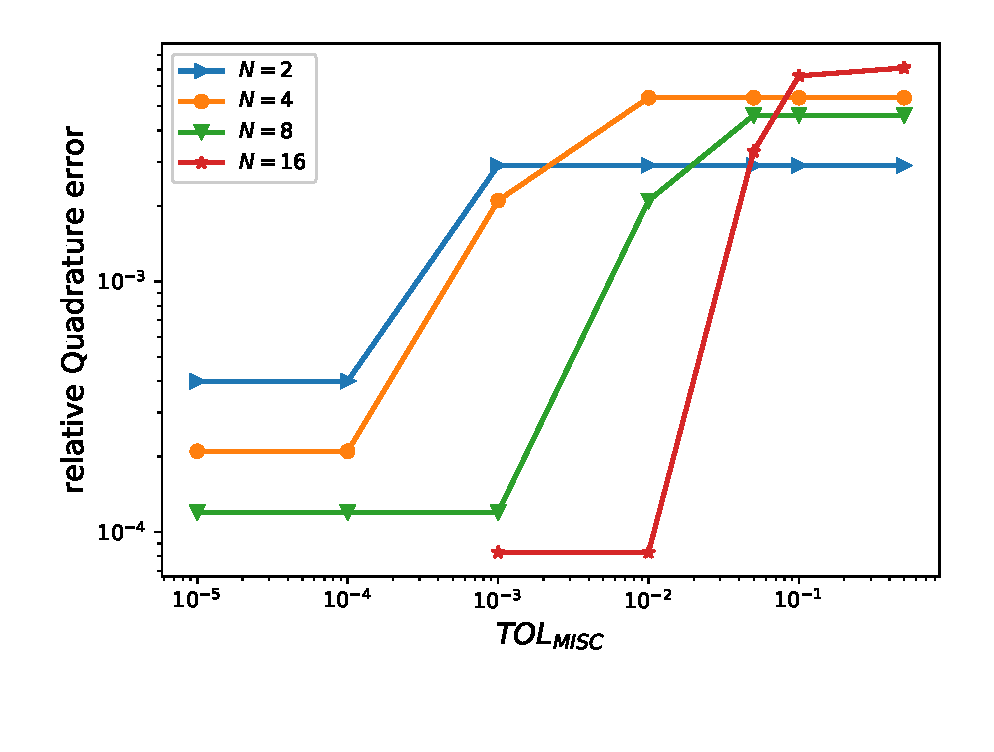
\includegraphics[width=0.35\linewidth]{./figures/rBergomi_MISC_quadratre_error/vs_TOL/set6/relative_quad_error_wrt_MISC_TOL_set6_non_rich}
%	
%	
%	\caption{Quadrature error of MISC, with different tolerances, to compute call option price  for different number of time steps. Case  set $3$ parameters, without Richardson extrapolation.}
%%	  See detailed values  in table \ref{Quadrature error of MISC to compute Call option price of the different tolerances for different number of time steps. Case  set $4$ parameters, without Richardson extrapolation. The numbers between parentheses are the corresponding absolute errors.}}
%	\label{fig:Quadrature_error_set4}
%\end{figure}
%
%
%
\FloatBarrier

\begin{table}[h!]
	\centering
	\begin{tabular}{l*{6}{c}r}
	\toprule[1.5pt]
	Method & & Steps  & &     \\
	\hline	
        & $2$ & $4$ & $8$ & $16$  \\
		\hline

		MISC ($\text{TOL}_{\text{MISC}}=10^{-1}$)  &  $\underset{(0.006,0.002)}{\mathbf{0.008}}$ & $\underset{(0.004,0.005)}{\mathbf{0.009}}$& $\underset{(0.003,0.005)}{\mathbf{ 0.008}}$ & $\underset{(0.002,0.007)}{\mathbf{ 0.009}}$   \\

		MISC ($\text{TOL}_{\text{MISC}}=10^{-2}$)  &  $\underset{(0.006,0.002)}{\mathbf{0.008}}$ & $\underset{(0.004,0.005)}{\mathbf{0.009}}$& $\underset{(0.003,0.002)}{\mathbf{ 0.005}}$ & $\underset{(0.002,1e-04)}{\mathbf{ 0.002}}$  \\
		MISC ($\text{TOL}_{\text{MISC}}=10^{-3}$)  &  $\underset{(0.006,0.002)}{\mathbf{0.008}}$& $\underset{(0.004,0.002)}{\mathbf{0.006}}$& $\underset{(0.003,1e-04)}{\mathbf{0.003}}$  & $\underset{(0.002,1e-04)}{\mathbf{ 0.002}}$  \\
		MISC ($\text{TOL}_{\text{MISC}}=10^{-4}$)  &  $\underset{(0.006,4e-04)}{\mathbf{0.006}}$ & $\underset{(0.004,2e-04)}{\mathbf{\red{0.004}}}$& $\underset{(0.003,1e-04)}{\mathbf{0.003}}$ & $\mathbf{ -}$ \\

		
		\hline
%		MC    & $\underset{(0.006,4e-04)}{\mathbf{0.006}}$  & $\underset{(0.004,4e-04)}{ \mathbf{0.004}}$  & $\underset{(0.003,4e-04)}{\mathbf{0.003}}$ & $\underset{(0.002,4e-04)}{\mathbf{0.002}}$  \\	
%		M(\# MC samples) 	& $5 \times 10^6$  & $5 \times 10^6$  & $5 \times 10^6$ & $5 \times 10^6$  \\
%		\hline
		MC    & $\underset{(0.006,0.005)}{\mathbf{0.01}}$  & $\underset{(0.004,0.004)}{ \mathbf{0.008}}$  & $\underset{(0.003,0.003)}{\mathbf{0.006}}$ & $\underset{(0.002,0.002)}{\mathbf{\red{0.004}}}$  \\	
		M(\# MC samples) 	& $2 \times 10^4$  & $4 \times 10^4$  & $6 \times 10^4$ & $8 \times 10^4$  \\
		\bottomrule[1.25pt]
	\end{tabular}
	\caption{Total relative error of MISC, without Richardson extrapolation, with different tolerances, and MC to compute the call option price  for different numbers of time steps. The values between parentheses correspond to the different errors contributing to the total relative error: for MISC we report the bias and quadrature errors and for MC we report the bias and the statistical errors estimates. The number of MC samples, $M$, is chosen to satisfy \eqref{optimal_number_samples}. The values marked in red correspond to the values used for computational work comparison against MC method, reported in Table \ref{table:Summary of our numerical results.}.}
	\label{Total error of MISC and MC to compute Call option price of the different tolerances for different number of time steps. Case set 4, without Richardson extrapolation. The numbers between parentheses are the corresponding absolute errors.}
\end{table}

\FloatBarrier
\begin{table}[h!]
	\centering
	\begin{tabular}{l*{6}{c}r}
	\toprule[1.5pt]
	Method & & Steps  & &     \\
	\hline	
		          & $2$ & $4$ & $8$ & $16$ &   \\
		\hline
%		MISC ($\text{TOL}_{\text{MISC}}=5.10^{-1}$)  & $0.1$ & $0.1$ & $0.1$ & $0.3$  \\
		MISC ($\text{TOL}_{\text{MISC}}=10^{-1}$)  & $0.1$ & $0.1$ & $0.1$ & $1$ \\
%		MISC ($\text{TOL}_{\text{MISC}}=5.10^{-2}$)  & $0.1$ & $0.1$ & $0.1$ & $22$  \\
		MISC ($\text{TOL}_{\text{MISC}}=10^{-2}$)  & $0.1$ & $0.15$ & $9$ & $112$ \\
		MISC ($\text{TOL}_{\text{MISC}}=10^{-3}$)  & $0.2$ & $2$ & $27$ & $2226$ \\
		MISC ($\text{TOL}_{\text{MISC}}=10^{-4}$)  & $1$ & $\red{6}$ & $136$ & $-$\\
%		MISC ($\text{TOL}_{\text{MISC}}=10^{-5}$)  & $2$ & $18$ & $1559$ & $-$
%		\\
%		\hline
%		MC method   & $ \red{141}
%		
%		$  & $  \red{246}$  & $  \red{461}$ & $ \red{820}
%		$  \\	
		\hline
		MC method   & $1
		
		$  & $ 3$  & $  10$ & $ \red{40}
		$  \\	
		\bottomrule[1.25pt]
%		Ratio of CPU time  $\left(MC/MISC \right)$ & $ \red{141}
%		
%		$  & $  \red{
%			41
%		}$  & $  \red{    17
%		}$ & $ \red{ 7}
%		$  \\	
%%		
%		\hline
	\end{tabular}
	\caption{Comparison of the computational time (in seconds) of  MC and MISC,  to compute the call option price of the rBergomi model for different numbers of time steps. The average  MC CPU time is computed over $100$ runs. The values marked in red correspond to the values used for computational work comparison against MC method, reported in Table \ref{table:Summary of our numerical results.}. }
	\label{Comparsion of the computational time of  MC and MISC, used to compute Call option price of rBergomi model for different number of time steps. Case set4}
\end{table}


\FloatBarrier

	\begin{figure}[h!]
	\centering
	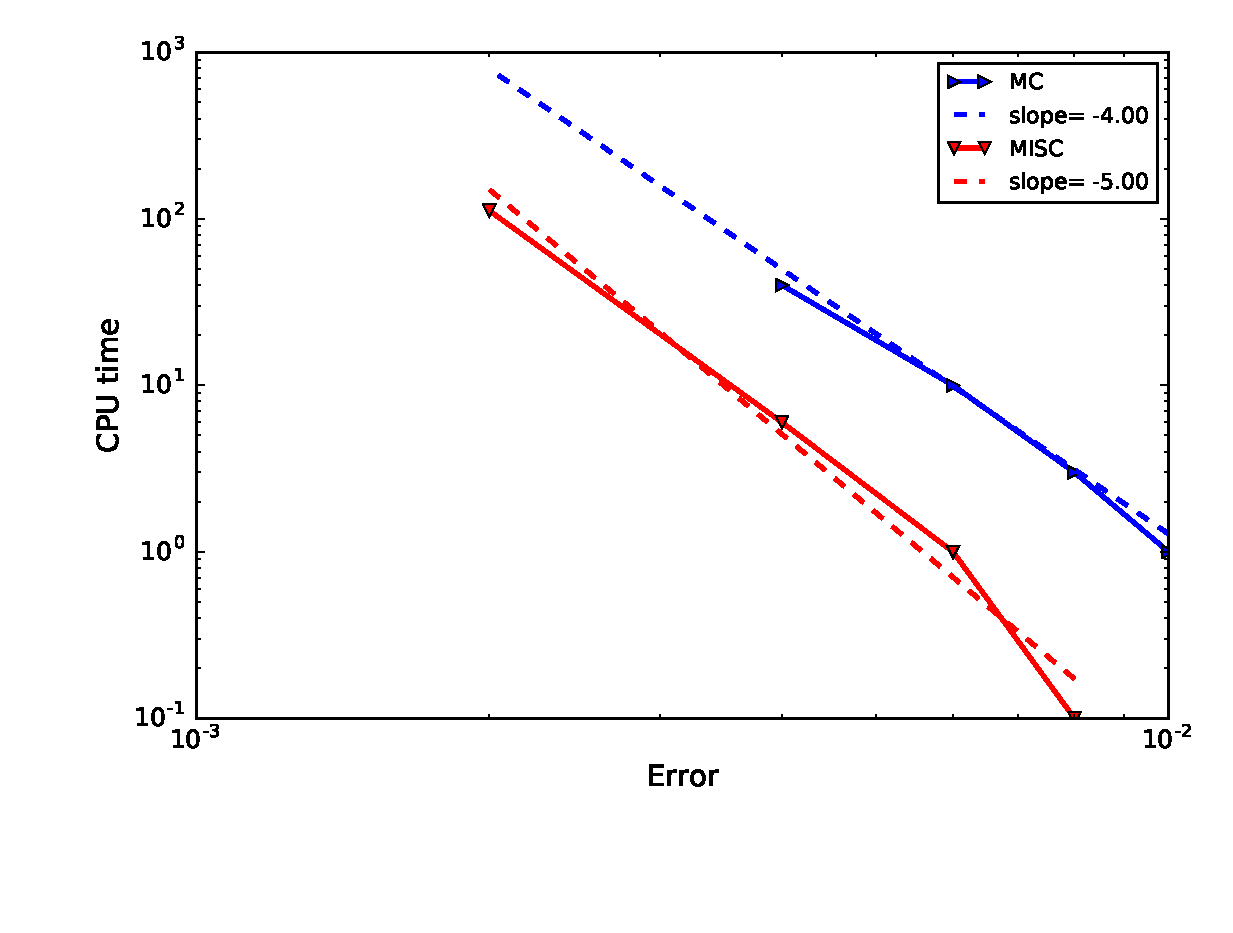
\includegraphics[width=0.5\linewidth]{./figures/rBergomi_Complexity_rates/set6/error_vs_time_set6_full_comparison}
	
	\caption{Comparison of computational work for MC and MISC methods, for the case of parameter set $3$ in Table \ref{table:Reference solution, using MC with $500$ time steps, of Call option price under rBergomi model, for different parameter constellation.}. This plot shows that to achieve a relative error below $1\%$, MISC outperforms MC method in terms of computational time.}
	\label{fig:Complexity plot for MC and MISC for case set $4$ parameters}
\end{figure}
\FloatBarrier
\subsubsection{Case of parameters in Set 4, in Table \ref{table:Reference solution, using MC with $500$ time steps, of Call option price under rBergomi model, for different parameter constellation.} }\label{sec:Case of set 5 parameters}

In this section, we only conduct our numerical experiments for the case without Richardson extrapolation. Our numerical experiments show that  MISC requires  approximately $75\%$ of the work of MC method, to achieve a total relative error of around $2\%$  (see Figure \ref{fig:Complexity plot for MC and MISC for Case set $5$ parameters} and Tables \ref{Comparsion of the computational time of  MC and MISC, used to compute Call option price of rBergomi model for different number of time steps. Case set5} and \ref{Total error of MISC and MC to compute Call option price of the different tolerances for different number of time steps. Case set 5, without Richardson extrapolation. The numbers between parentheses are the corresponding absolute errors.}). Similar to the case of set $1$ parameters illustrated in section \ref{sec:Case of set $2$ parameters_linear}, we believe that Richardson extrapolation will improve the performance of MISC method.   

%\FloatBarrier
%\begin{table}[h!]
%	\centering
%	\begin{tabular}{l*{6}{c}r}
%		Method \textbackslash  Steps            & $2$ & $4$ & $8$ & $16$ &   \\
%		\hline
%%		MISC ($\text{TOL}_{\text{MISC}}=5.10^{-1}$)  & $0.0590$ & $0.0564$ & $0.0552$ & $0.0546$  \\
%		MISC ($\text{TOL}_{\text{MISC}}=10^{-1}$)  & $0.0590$ &$0.0564$& $0.0552$ & $0.0546$   \\
%%		MISC ($\text{TOL}_{\text{MISC}}=5.10^{-2}$)  &$0.0590$ & $0.0564$ & $0.0552$ & $0.0557$  \\
%		MISC ($\text{TOL}_{\text{MISC}}=10^{-2}$)  &$0.0590$ &$0.0564$ & $0.0574$ & $0.0572$  \\
%		
%		MISC ($\text{TOL}_{\text{MISC}}=10^{-3}$)  & $0.0605$ & $0.0587$ & $0.0579$ & $0.0575$  \\
%%		MISC ($\text{TOL}_{\text{MISC}}=10^{-4}$)  &  $0.0605$ & $0.0587$ & $0.0576$ & $-$  \\
%%		
%%		MISC ($\text{TOL}_{\text{MISC}}=10^{-5}$)  & $0.0605$ & $0.0587$ &  $0.0579$ & $-$  \\
%		\hline
%		MC method ($M=5.10^{6}$)   & $0.0605$ & $0.0587$  & $0.0579$ & $0.0576$ \\		
%		
%		\hline
%	\end{tabular}
%	\caption{ Call option price of the different methods for different number of time steps. Case of set $5$ parameters in table \ref{table:Reference solution, using MC with $500$ time steps, of Call option price under rBergomi model, for different parameter constellation.}, without Richardson extrapolation.}
%	\label{table: Call option price of the different methods for different number of time steps. Case set 5}
%\end{table}

%\FloatBarrier
%\begin{table}[h!]
%	\centering
%	\begin{tabular}{l*{6}{c}r}
%		Method \textbackslash  Steps            & $2$ & $4$ & $8$ & $16$  \\
%		\hline
%		MC Bias ($M=5.10^6$)   & 	$ \underset{(0.0037
%			)}{\mathbf{0.0650}}$  & $\underset{(0.0019)}{\mathbf{0.0330
%		}}$  & $\underset{(0.0012)}{\mathbf{0.0202}}$ & $\underset{(0.0007)}{\mathbf{0.0130}}$\\ 
%		
%		MC Statistical error ($M=5.10^6$)  &  $\underset{(   4.0e-05)} {\mathbf{7.0e-04}}$  & $\underset{(3.8e-05)} {\mathbf{6.7e-04}}$  & $\underset{(3.7e-05)} {\mathbf{6.5e-04 }}$ & $\underset{(3.6e-05)} {\mathbf{6.3e-04}}$	\\
%		
%		\hline
%	\end{tabular}
%	\caption{Bias and statistical errors of MC   for computing call option price  for different number of time steps. Case set $4$, without Richardson extrapolation. The numbers between parentheses are the corresponding absolute errors.}
%	\label{Bias and Statistical errors of MC ($M=5.10^6$)  for computing Call option price  for different number of time steps. Case set 5, without Richardson extrapolation. The numbers between parentheses are the corresponding absolute errors.}
%\end{table}
%%
%%
%%
%
%
%\FloatBarrier





%\begin{figure}[h!]
%	\centering
%	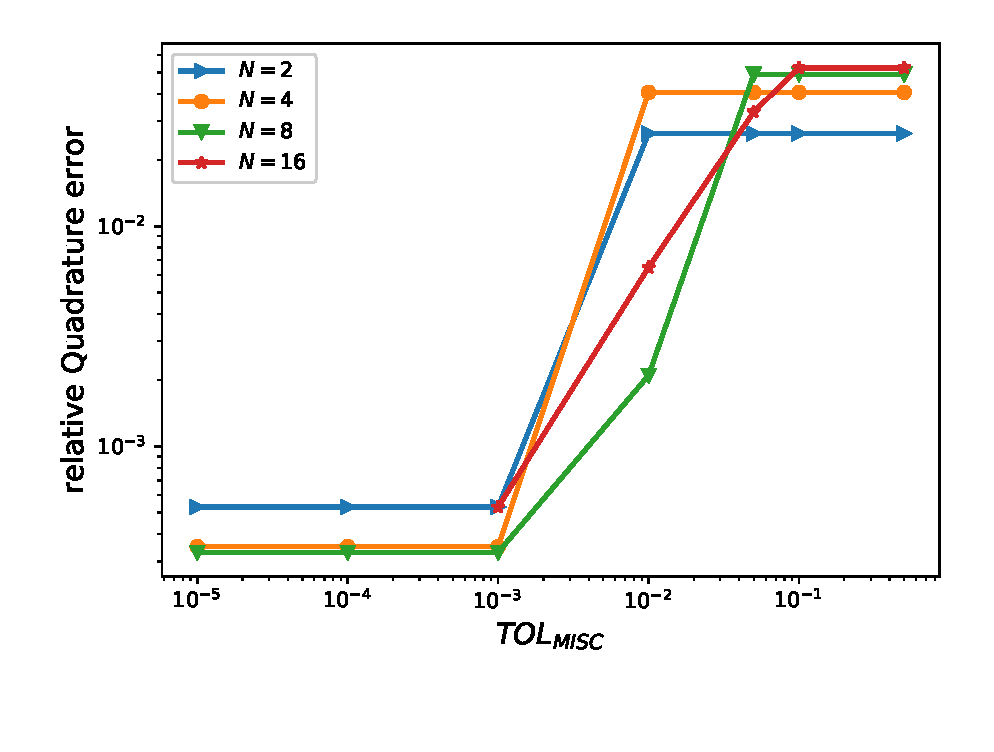
\includegraphics[width=0.35\linewidth]{./figures/rBergomi_MISC_quadratre_error/vs_TOL/set7/relative_quad_error_wrt_MISC_TOL_set7_non_rich}
%	
%	
%	\caption{Quadrature error of MISC, with  different tolerances,  to compute call option price  for different number of time steps. Case  set $4$ parameters, without Richardson extrapolation. }
%%	 See detailed values  in table \ref{Quadrature error of MISC to compute Call option price of the different tolerances for different number of time steps. Case  set $5$ parameters, without Richardson extrapolation. The numbers between parentheses are the corresponding absolute errors.}}
%	\label{fig:Quadrature_error_set5}
%\end{figure}
%
%\FloatBarrier
%%
%
%
\begin{table}[h!]
	\centering
	\begin{tabular}{l*{6}{c}r}
	\toprule[1.5pt]
	Method & & Steps  & &     \\
	\hline	
		         & $2$ & $4$ & $8$ & $16$  \\
		\hline

		MISC ($\text{TOL}_{\text{MISC}}=10^{-1}$)  & $\underset{(0.07,0.05)}{\mathbf{0.09}}$ & $\underset{(0.03,0.04)}{\mathbf{0.07}}$& $\underset{(0.02,0.05)}{\mathbf{ 0.07}}$ & $\underset{(0.01,2e-04)}{\mathbf{ 0.06}}$   \\

		MISC ($\text{TOL}_{\text{MISC}}=10^{-2}$)  &  $\underset{(0.07,5e-04)}{\mathbf{0.09}}$& $\underset{(0.03,0.04)}{\mathbf{0.07}}$& $\underset{(0.02,3e-04)}{\mathbf{ \red{0.02}}}$ & $\underset{(0.01,2e-04)}{\mathbf{ 0.02}}$  \\
		MISC ($\text{TOL}_{\text{MISC}}=10^{-3}$)  &  $\underset{(0.07,5e-04)}{\mathbf{0.07}}$& $\underset{(0.03,4e-04)}{\mathbf{0.03}}$& $\underset{(0.02,3e-04)}{\mathbf{0.02}}$  & $\underset{(0.01,2e-04)}{\mathbf{ 0.01}}$  \\
%
%		\hline
%		MC    & $\underset{(0.07,7e-04)}{\mathbf{0.07}}$  & $\underset{(0.03,6e-04)}{\mathbf{0.03}}$  & $\underset{(0.02,6e-04)}{\mathbf{0.02}}$ & $\underset{(0.01,6e-04)}{\mathbf{0.01}}$  \\		
%			M(\# MC samples)   & $5 \times 10^6$  & $5 \times 10^6$  & $5 \times 10^6$ & $5 \times 10^6$  \\		
			\hline
		MC    & $\underset{(0.07,0.07)}{\mathbf{0.14}}$  & $\underset{(0.03,0.04)}{\mathbf{0.07}}$  & $\underset{(0.02,0.02)}{\mathbf{0.04}}$ & $\underset{(0.01,0.01)}{\mathbf{\red{0.02}}}$  \\		
			M(\# MC samples)   & $6 \times 10^2$  & $2 \times 10^3$  & $8 \times 10^3$ & $2 \times 10^4$  \\		
		\bottomrule[1.25pt]
	\end{tabular}
	\caption{Total relative error of MISC, without Richardson extrapolation, with  different tolerances,  and MC to compute the call option price  for different numbers of time steps. The values between parentheses correspond to the different errors contributing to the total relative error: for MISC we report the bias and quadrature errors and for MC we report the bias and the statistical errors estimates. The number of MC samples, $M$, is chosen to satisfy \eqref{optimal_number_samples}. The values marked in red correspond to the values used for computational work comparison against MC method, reported in Table \ref{table:Summary of our numerical results.}.}
	\label{Total error of MISC and MC to compute Call option price of the different tolerances for different number of time steps. Case set 5, without Richardson extrapolation. The numbers between parentheses are the corresponding absolute errors.}
\end{table}

\FloatBarrier
\begin{table}[h!]
	\centering
	\begin{tabular}{l*{6}{c}r}
	\toprule[1.5pt]
	Method & & Steps  & &     \\
	\hline	
		        & $2$ & $4$ & $8$ & $16$ &   \\
		\hline
%		MISC ($\text{TOL}_{\text{MISC}}=5.10^{-1}$)  & $0.1$ & $0.1$ & $0.2$ & $0.5$  \\
		MISC ($\text{TOL}_{\text{MISC}}=10^{-1}$)  & $0.1$ & $0.1$ & $0.2$ & $0.5$ \\
%		MISC ($\text{TOL}_{\text{MISC}}=5.10^{-2}$)  & $0.1$ & $0.1$ & $0.2$ & $5$  \\
		MISC ($\text{TOL}_{\text{MISC}}=10^{-2}$)  & $0.1$ & $0.1$ & $\red{8}$ & $97$ \\
		MISC ($\text{TOL}_{\text{MISC}}=10^{-3}$)  & $0.7$ & $4$ & $26$ & $1984$ \\
%		MISC ($\text{TOL}_{\text{MISC}}=10^{-4}$)  & $1$ & $8$ & $173$ & $-$\\
%		MISC ($\text{TOL}_{\text{MISC}}=10^{-5}$)  & $1$ & $32$ & $2129$ & $-$
%		\\
%		\hline
%		MC method   & $ \red{154}
%		
%		$  & $  \red{229}$  & $  \red{420}$ & $ \red{938}
%		$  \\	
		\hline
		MC method   & $ 0.02
		
		$  & $  0.15$  & $ 1.4$ & $ \red{10}$  \\	
	\bottomrule[1.25pt]
%		Ratio of CPU time  $\left(MC/MISC \right)$ & $ \red{   220}
%		
%		$  & $  \red{
%		 57
%		}$  & $  \red{    16
%		}$ & $ \red{ 0.5}
%		$  \\	
%				
%		\hline
	\end{tabular}
	\caption{Comparison of the computational time (in seconds) of  MC and MISC, to compute the call option price of rBergomi model for different numbers of time steps. The average  MC CPU time is computed over $100$ runs. The values marked in red correspond to the values used for computational work comparison against MC method, reported in Table \ref{table:Summary of our numerical results.}. }
	\label{Comparsion of the computational time of  MC and MISC, used to compute Call option price of rBergomi model for different number of time steps. Case set5}
\end{table}

\FloatBarrier


	\begin{figure}[h!]
	\centering
	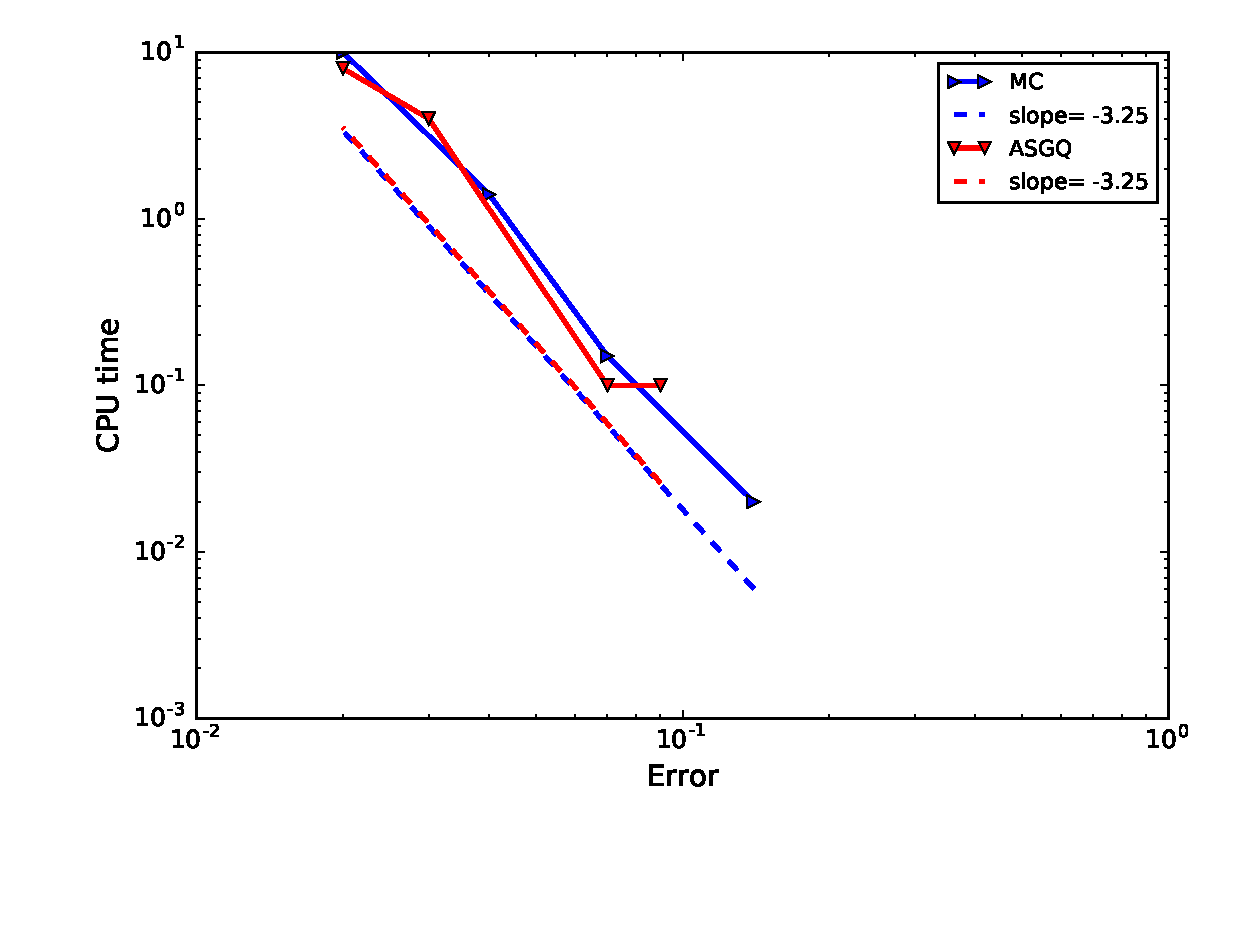
\includegraphics[width=0.5\linewidth]{./figures/rBergomi_Complexity_rates/set7/error_vs_time_set7_full_comparison}
	
	\caption{Comparison of computational work for MC and MISC methods, for the case of parameter set $4$ in Table \ref{table:Reference solution, using MC with $500$ time steps, of Call option price under rBergomi model, for different parameter constellation.}. This plot shows that to achieve a relative error around $1\%$, MISC and  MC methods have similar performance in terms of computational time.}
	\label{fig:Complexity plot for MC and MISC for Case set $5$ parameters}
\end{figure}
\FloatBarrier


